\documentclass[a4paper,10pt,review]{elsarticle}

\usepackage{lineno,hyperref}
\modulolinenumbers[5]

% START: Inserted by AJS
\frenchspacing
\usepackage{ifxetex}
\ifxetex
  \usepackage{fontspec}
  \defaultfontfeatures{Ligatures=TeX} % To support LaTeX quoting style
  \setromanfont{Hoefler Text}
  % \setmainfont[Ligatures=TeX]{Palatino}
\else
  \usepackage[T1]{fontenc}
  \usepackage[utf8]{inputenc}
  \usepackage{lmodern}
  \usepackage{textcomp} % directly use the degree (and some other) symbol
\fi

\usepackage{fixltx2e}
\usepackage[]{graphicx}
\usepackage{wrapfig}
\usepackage{lscape}
\usepackage{rotating}
\usepackage{epstopdf}
\usepackage{ragged2e}  % for '\RaggedRight' macro (allows hyphenation)
\usepackage[pdftex]{color}
\usepackage[margin=2.75cm]{geometry}
\usepackage{upquote}
\usepackage{textgreek}
\usepackage{microtype} % place after fonts; even better typesetting for improved readability
\usepackage{xfrac} % nice fractions
\usepackage{booktabs} % nice tables without vertical lines
\setlength\heavyrulewidth{0.1em}
\setlength\lightrulewidth{0.0625em}
\usepackage[color=yellow, textsize=tiny]{todonotes}
\usepackage[font={small}, labelfont=bf]{caption} % tweaking the captions
\usepackage{gensymb}
\usepackage{amsmath,amssymb}
\usepackage{cleveref} % clever cross referencing figures and tables; last package to include
% END: Inserted by AJS
\usepackage{natbib}

\journal{Progress in Oceanography}

%%%%%%%%%%%%%%%%%%%%%%%
%% Elsevier bibliography styles
%%%%%%%%%%%%%%%%%%%%%%%
%% To change the style, put a % in front of the second line of the current style and
%% remove the % from the second line of the style you would like to use.
%%%%%%%%%%%%%%%%%%%%%%%

%% Numbered
%\bibliographystyle{model1-num-names}

%% Numbered without titles
% \bibliographystyle{model1a-num-names}

%% Harvard
% \bibliographystyle{model2-names.bst}\biboptions{authoryear}

%% Vancouver numbered
%\usepackage{numcompress}\bibliographystyle{model3-num-names}

%% Vancouver name/year
% \usepackage{numcompress}\bibliographystyle{model4-names}\biboptions{authoryear}

%% APA style
% \bibliographystyle{model5-names}\biboptions{authoryear}

%% AMA style
%\usepackage{numcompress}\bibliographystyle{model6-num-names}

%% `Elsevier LaTeX' style
% \bibliographystyle{elsarticle-num}
\bibliographystyle{elsarticle-harv}\biboptions{authoryear}
% \bibliographystyle{elsarticle-num-names}
%%%%%%%%%%%%%%%%%%%%%%%

\begin{document}

\begin{frontmatter}

\title{Nearshore and offshore co-occurrence of marine heatwaves and cold-spells}

%% or include affiliations in footnotes:
\author[firstaddress]{Robert W. Schlegel\corref{mycorrespondingauthor}}
\cortext[mycorrespondingauthor]{Corresponding author}
\ead{3503570@myuwc.ac.za}
\author[secondaddress,thirdaddress]{Eric C. J. Oliver}
\author[fourthaddress]{Thomas Wernberg}
\author[firstaddress]{Albertus J. Smit}


% \author[mysecondaryaddress]{Global Customer Service\corref{mycorrespondingauthor}}

\address[firstaddress]{Department of Biodiversity and Conservation Biology, University of the Western Cape, Private Bag X17, Bellville 7535, South Africa}

\address[secondaddress]{ARC Centre of Excellence for Climate System Science, Australia}

\address[thirdaddress]{Institute for Marine and Antarctic Studies, University of Tasmania, Hobart, Australia}

\address[fourthaddress]{UWA Oceans Institute and School of Plant Biology, The University of Western Australia, Crawley, 6009 Western Australia, Australia}

\begin{abstract}
A changing global climate places shallow water ecosystems at more risk than those in the open ocean as their temperatures may change more rapidly and dramatically. To this end, it is necessary to identify the occurrence of extreme ocean temperature events --- marine heatwaves (MHWs) and marine cold-spells (MCSs) --- in the nearshore environment as they can have lasting ecological effects. The occurrence of MHWs have been investigated regionally, but no investigations of MCSs have yet to be carried out. A recently developed framework that defines these events in a novel way was applied to ocean temperature time series from i) a nearshore \emph{in situ} dataset and ii) \sfrac{1}{4}\degree~NOAA Optimally Interpolated sea surface temperatures. Regional drivers due to nearshore influences (local-scale) and the forcing of two offshore ocean currents (broad-scale) on MHWs and MCSs were taken into account when the events detected in these two datasets were used to infer the links between offshore and nearshore temperatures in time and space. We show that MHWs and MCSs occur at least once a year on average but that proportions of co-occurrence of events between the broad- and local scales are low (0.20-0.50), with MHWs having greater proportions of co-occurrence than MCSs. The low rates of co-occurrence between the nearshore and offshore datasets show that drivers other than mesoscale ocean temperatures play a role in the occurrence of at least half of nearshore events. Significant differences in the duration and intensity of events between different coastal sections may be attributed to the effects of the interaction of oceanographic processes offshore, as well as with local features of the coast. The regional decadal trends in the occurrence of MHWs and MCSs in the offshore dataset show that generally MHWs are increasing there while MCSs are decreasing. This study represents an important first step in the analysis of the dynamics of events in nearshore environments, and their relationship with broad-scale influences.
\end{abstract}

\begin{keyword}
extreme events \sep co-occurrence \sep remotely-sensed SST \sep \emph{in situ} data \sep climate change \sep coastal
\end{keyword}

\end{frontmatter}

\linenumbers

\section{Introduction}
Over the past three decades, anthropogenically mediated warming has negatively affected marine and terrestrial ecosystems with far reaching consequences for humanity and natural ecological functioning. Although climate change is generally understood as a gradual long-term rise in global mean surface temperature \citep{IPCC2014}, which will continue for decades or centuries, it is generally the associated increase in frequency and severity of extreme events that affects humans and ecosystems in the short-term \citep{Easterling2000}. Impacts of extreme events such as floods, wind storms, tropical cyclones, heatwaves and cold-spells are often sudden with catastrophic consequences. The recognition to focus more on the extremes and less on the background mean state has emerged as a critical direction of climate change research \citep{Jentsch2007}.

`Heatwaves' usually refer to atmospheric phenomena where vague definitions such as ``a period of abnormally and uncomfortably hot [...] weather'' are invoked \citep{Glickman2000}, but there are also precise definitions based on statistical properties and other metrics of the temperature record that are relative to location and time of year \citep[e.g.][]{Meehl2004, Alexander2006, Fischer2010, Fischer2011, Perkins2013}. As the definitions for heatwaves have increased, so to have the investigations of heatwaves in the ocean \citep[e.g.][]{Mackenzie2007, Selig2010, Sura2011, Lima2012, DeCastro2014}. Well-known marine heatwaves (MHWs) have occurred in the Mediterranean in 2003 \citep{Black2004, Olita2007, Garrabou2009}, off the coast of Western Australia in 2011 \citep{Feng2013, Pearce2013, Wernberg2013}, in the north west Atlantic Ocean in 2012 \citep{Mills2012, Chen2014, Chen2015} and more recently the ``Blob'' in the north east Pacific Ocean \citep{Bond2015}. The extreme temperatures from these events have had negative impacts on the local ecology of the regions in which they occur. For example, the 2003 Mediterranean heatwave may have affected up to 80\% of the gorgonian fan colonies in some areas \citep{Garrabou2009}, and the 2011 event off the west coast of Australia is now known to have caused a 100 km range contraction of temperate kelp forests in favor of seaweed turfs and a tropicalisation of reef fishes \citep{Wernberg2016}.

Although the consequences of these anomalously warm events have been widely publicized, the events themselves have until recently not been objectively characterized. In part, this has been due to the lack of a consistent definition and metrics. In response to this need, \citet{Hobday2016} developed a definition of a MHW as ``a prolonged discrete anomalously warm water event that can be described by its duration, intensity, rate of evolution, and spatial extent,'' and in doing so have derived statistical metrics that quantify these properties. For example, the count of MHWs within a time series and their maximum and cumulative intensity are quantifiable parameters that can be calculated in a consistent manner irrespective of geographical location. The focus of this paper is on marine thermal events that are anomalous with respect to the seasonal climatology as per the \citet{Hobday2016} definition. They may be anomalously warm events, or anomalously cold (marine cold-spells, MCSs; introduced here). While MHWs are becoming reasonably well known by virtue of their increasing count and intensity, MCSs have received less recognition. Whereas extreme hot events may be demonstrably damaging to organisms and ecosystems, extreme cold events also have the potential to negatively impact organisms and ecosystems \citep{Lirman2011}. In both cases their drivers and dynamics, particularly in the nearshore (<400 m from the coastline), remain poorly understood.

MCSs are projected to become less frequent under future climatic scenarios, but there are also examples of them becoming more frequent in some localities \citep[e.g.][]{Gershunov2008, Matthes2015}. They are frequently lethal to marine organisms \citep{Woodward1987} and are known to have caused mass fish \citep{Gunter1941, Gunter1951, Holt1983} and invertebrate \citep{Gunter1951, Crisp1964} kills, the death of juvenile and sub-adult manatees \citep{OShea1985, Marsh1986} and coral bleaching \citep{Lirman2011}. Cold temperatures are very important in setting species population distribution limits, particularly limiting their range north- or southwards towards higher latitudes \citep{Firth2011}, and the timing of the onset of growing seasons \citep{Jentsch2007}. It is easy to imagine how population-level consequences might aggregate to drive whole ecosystem responses \citep[e.g.][]{Kreyling2008, Rehage2016}. Indeed, the range contractions of ecosystem engineer species such as mussels have been shown to relate to MCSs \citep{Firth2011, Firth2015}.

Although we understand that the sea surface temperature (SST) of the upper mixed layer is influenced by oceanic and atmospheric processes \citep[see Equation 1 of][]{Deser2010}, there is by no means a good understanding of how these processes are modulated by local- \emph{vs.} broad-scale influences, thus resulting in nearshore MHWs and MCSs. Some of the MCSs known to have impacted populations were caused by atmospheric cold-spells affecting the intertidal and coastal biota locally \citep{Gunter1941, Firth2011}. We hypothesise that these localized events are manifestations of extreme atmospheric cold weather phenomena situated over the coast resulting in rapid heat loss from coastal waters. On the other hand, we also hypothesize that broader-scale teleconnections may also affect the thermal properties and dynamics of coastal systems. For example, large-scale atmospheric-oceanographic coupling is being affected by global warming, which is projected to cause the intensification of upwelling favorable winds and consequently the intensification and increasing count of upwelling events \citep[see][for a review of this and alternative hypotheses]{Garcia-Reyes2015}. It is therefore possible that the development of \emph{some} nearshore MCSs may be attributed to an intensification of upwelling. MHWs at any scale likely originate directly from atmosphere-ocean heat transfer as in the Mediterranean Sea \citep[e.g.][]{Garrabou2009} or from advection, i.e., the transport of warm water due to currents such as what happened off Western Australia in 2011 \citep{Feng2013, Benthuysen2014}, the NW Atlantic in 2012 \citep{Mills2012, Chen2014, Chen2015} and potentially off SE Australia in 2016. Because MHWs and MCSs are both able to affect ecosystem change, a mechanistic understanding of their drivers may be useful for conservation and management purposes. To this end our study serves as a constructive first step to understand the prevalence of anomalous thermal events with respect to forcing mechanisms at different scales.

\citet{Hobday2016} applied their MHW framework to the \sfrac{1}{4}\degree~NOAA Optimally Interpolated SST dataset \citep[hereafter referred to as OISST;][]{Reynolds2007}, but warned users to be cognizant that different data sets would provide different kinds of information pertaining to heatwaves. Our study applied this MHW (MCS) definition to datasets of nearshore \emph{in situ} (local-scale) and offshore gridded OISST (broad-scale) temperature time series collected at different locations along coastlines influenced by contrasting ocean currents --- the Benguela Current, an eastern boundary upwelling system, and the Agulhas Current --- and locally modified by regional aspects of the coastal bathymetry, geomorphology and other smaller scale coastal features. Having assessed these systems within a framework that coupled local- and broad-scale features permitted us to assess how MHWs (MCSs) developed in coastal regions. Specifically, we aimed to assess the significance of MHWs (MCSs) within the context of the datasets’ inherent differences, and examine the various dynamical properties that then emerged out of the regional oceanographic context and out of the local-scale modifications of the regional ocean features as they approached the coast. In doing so, the aim was to provide some insights into possible mechanisms that determine the nature and origin of MHWs (MCSs) within regionally distinct ocean/ coastal sections. We hypothesized that i) nearshore local-scale MHW events are coupled with offshore broad-scale thermal patterns; ii) MCSs originate at the local-scale in the nearshore \emph{in situ} dataset as isolated incidents decoupled from broader-scale patterns; iii) different coastal sections, each variously influenced by interactions between local- and broad-scale processes, display different dynamics (timing, count, duration and intensity) of MHWs (MCSs); and iv) the count of warm (cold) events increases (decreases) with time under a regime of climate change. The effect of atmospheric forcing on nearshore events was considered but not assessed within the scope of this study.

\section{Methods}
\subsection{Study region}
The variety of oceanographic features around the \emph{ca}. 2,700 km long South African coast provides a natural laboratory for the potential effects of different ocean forcing mechanisms on the occurrence of MHWs and MCSs. Annual mean (± standard deviation; SD) coastal seawater temperatures range from 12.3±1.2\degree C at the western limit near the Namibian border (Site 1) to 24.4±2.0\degree C in the east near the Mozambican border (Site 21). Our study sites covered this full range (\Cref{fig:Figure1}). We classified the coast into three regions based on their major oceanographic features, their temperature characteristics, and aspects of the underlying continental shelf. The west coast region is dominated by the Benguela Current, which forms an Eastern Boundary Upwelling System (EBUS) \citep{Hutchings2009}. Seasonal upwelling is maintained by prevailing south-easterly trade winds and low temperatures are especially noticeable at upwelling cells over a relatively narrow continental shelf in the region from the Cape Peninsula to Cape Columbine. The west coast represents a cool temperate regime, with the range of monthly mean temperatures at most sections intermediate between cold temperate and warm temperate \citep{Luning1990}. The warm temperate east coast region is strongly influenced by the warm south-westerly flowing Agulhas Current, which hugs tightly along the narrow continental shelf (except for the Natal Bight) \citep{Luning1990}. This stretch of coast is spatially homogeneous with respect to temperature and characterized by a moderate amount of seasonal variation. Although the Agulhas Current retroflects back into the southern Indian Ocean \citep{Hutchings2009} just south of the much wider and cooler Agulhas Bank \citep{Roberts2005}, its influence regularly extends as far west as False Bay (Sites 5--21; \Cref{fig:Figure1}). Between the west and east coasts is the south coast region overlying the Agulhas Bank. Although also warm temperate, the south coast is fundamentally different from the other coastal sections in that it is dominated by not one strong current, but rather consists of a broad continental shelf on which the interplay of the Agulhas and Benguela Currents form a `mixing-pot' between two oceans, as well as hosting an attendant array of complex coastal processes that modify the already thermally variable waters overlying the Agulhas Bank \citep{Lutjeharms2003, Roberts2005, Hutchings2009}. It experiences a much larger range in annual temperature and variability compared to the west and east coast regions, which is in part influenced by the retention and cooling of Agulhas Current water on the bank, the presence of some current-driven upwelling cells along this coastal section (Sites 15--17) \citep{Roberts2005}, and from the effects of capes and embayments throughout the region. A more detailed description of these three coastal regions may be found in \citet{Smit2013}.

\begin{figure}
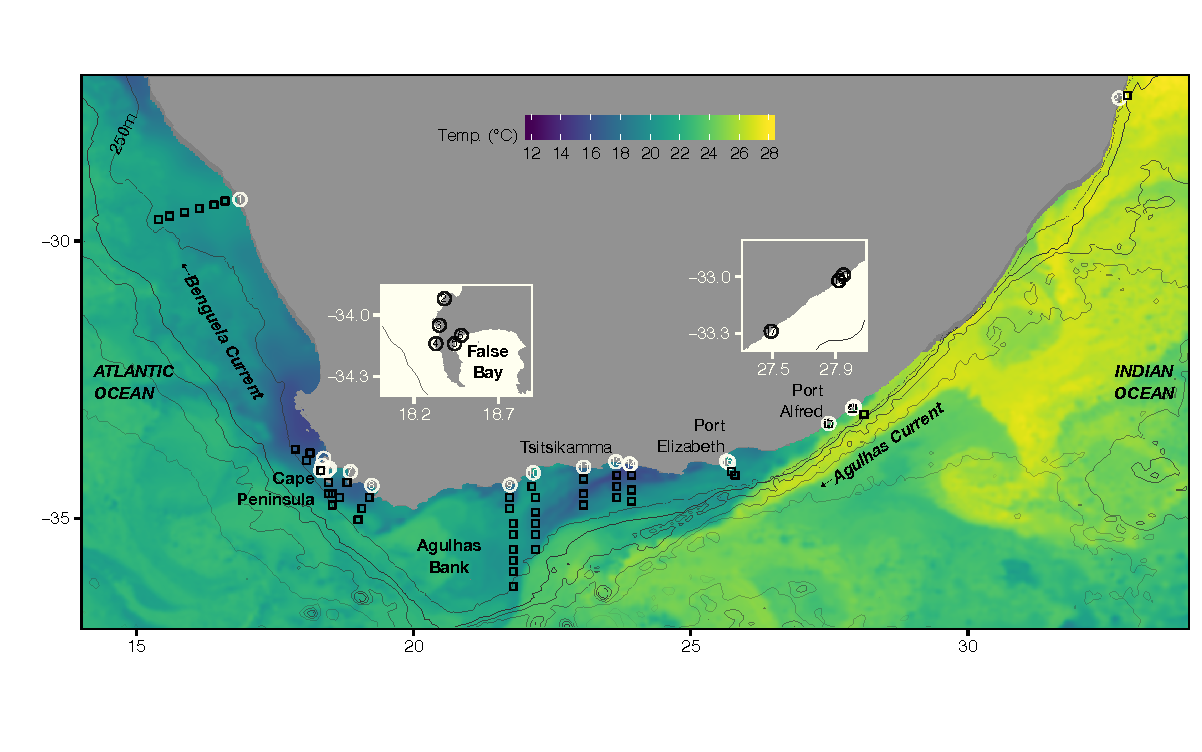
\includegraphics[width=1.0\textwidth]{figure1_1km_inset_map_labeled.pdf}
\caption{Map of southern Africa showing the bathymetry (only the 250m isobath is labelled), the location of the \emph{in situ} temperature time series shown with circles and approximations of the pixels used along the shore-normal transects from the daily \sfrac{1}{4}\degree~NOAA OISST \citep{Reynolds2007} shown with black boxes. The JPL G1SST 1 km blended SST field shows the state of the ocean on 2016-02-14; this image was selected as it clearly shows the full range of ocean processes around southern Africa. The Agulhas Current along the east coast of the country (Sites 18--21) is visualized here in a yellowish color as a jet of relatively warmer water projecting in a south-westerly direction, and hugging the continental shelf. The blueish patches north of the Cape Peninsula along the west coast (Sites 1--4) represent upwelled water. Some upwelled water on the south coast (Sites 5--17) may also be present around Sites 14 (Tsitsikamma) and 15--16 (Port Elizabeth). The inset maps show detail of the Cape Peninsula/ False Bay area and the Port Alfred region where site labels are obscured due to overplotting of symbols.}
\label{fig:Figure1}
\end{figure}

\subsection{Temperature data}
The \emph{in situ} seawater temperature dataset used in this study was comprised of 127 records of daily measurements of up to 40 years with a mean duration of \emph{ca}. 19 years. These \emph{in situ} time series are generally shorter than the recommended 30 year minimum for the characterization of MHWs \citep{Hobday2016} and have occasional gaps of missing data. However, there is a clear benefit of using \emph{in situ} data over satellite data as they provide a more accurate representation of the the thermal characteristics near the coast where satellite measurements do not capture maximum and minimum temperatures well \citep[e.g.][]{Smale2009, Castillo2010}. For example, satellite SST data along the coast of South Africa have shown warm biases as high as 6\degree C over \emph{in situ} temperatures in the nearshore environment \citet{Smit2013}. All time series from the \emph{in situ} dataset under 10 years in duration were excluded from this study to ensure at least one decade of data was used to estimate the climatology required for the identification of MHWs (MCSs). Time series missing more than 10\% of their daily temperature measurements were also excluded, leaving a total of 21 time series. These were then classified into the three coastal regions detailed above. Metadata for the selected time series, including location, duration, and the coastal regions they were aggregated into can be found in \Cref{tableS1}.

The remotely sensed temperature dataset used in this study were the daily \sfrac{1}{4}\degree~NOAA Optimally Interpolated SST \citep[OISST;][]{Reynolds2007} derived from the Advanced Very High Resolution Radiometer (AVHRR). To create time series from these OISST data representing offshore mesoscale temperatures and also comparable against the \emph{in situ} time series, shore-normal transects were drawn from each of the 21 sites extending to the 200m isobath. Temperature values from the OISST data were then extracted at each of the roughly 25~\texttimes~25 km pixels along these transects, shown as black boxes in \Cref{fig:Figure1}. Where the shelf was less than 25 km wide (Sites 17--21) the nearest `ocean pixel' to the \emph{in situ} time series coordinate was used. The daily temperatures for each pixel from the OISST dataset within each of the 21 shore-normal transects were meaned to create offshore time series that could be compared against the nearshore \emph{in situ} time series from which each transect was drawn. Offshore transects were used to generate the time series this way as they better represent the mesoscale temperatures we were interested in comparing against the coastal events. Had we simply used the nearest OISST pixel to generate time series to compare against the \emph{in situ} data this would only draw a comparison between the two different data types at the coast, and not the mesoscale activity in the ocean. These 21 OISST time series could then be analysed for MHWs (MCSs) in the same way as the \emph{in situ} data (see below). Note that the OISST time series had valid data covering 1982--2015 which did not match exactly with the individual \emph{in situ} sites.

\subsection{Defining and calculating MHWs and MCSs}
MHWs are defined here following \citet{Hobday2016} as ``discrete prolonged anomalously warm water events in a particular location.'' MCS are defined in the same manner as MHWs with the exception of being ``anomalously cold water events''.

To detect anomalous events, a climatological mean and 90th and 10th percentiles were first calculated for each day of the year within each time series by pooling all data within an 11-day window across all years. An 11 day window was chosen to ensure a robust estimate of the climatological mean as well as the 90th and 10th percentile thresholds. MHWs (MCSs) were detected as periods of time when temperatures exceeded (fell below) the 90th (10th) percentile for at least five days. The 90th (10th) percentile was used rather than the 95th (5th) or 99th (1st) so as to allow for the detection of a greater number of anomalous events. This is an important consideration as it is not only the very largest events that may pose a threat to local ecosystems. Starting from the 3 day minimum duration set for atmospheric heatwaves in \citet{Perkins2013}, different minimum lengths for the definition of marine events were tested for by \citet{Hobday2016}. They found that a minimum length of 5 days allowed for more uniform global results in event detection; therefore, we have used this 5 day minimum length in our study, too. Because our \emph{in situ} time series were of differing durations, with many under the proscribed 30 years, we calculated the climatology over all available years; in the case of the OISST data, climatologies were calculated over a fixed 33-year base period (1982--2015). Furthermore, discrete events with well-defined start and end dates but with `breaks' between events lasting $\leq$2 days followed by subsequent $\geq$5 day events were considered as continuous events \citep{Hobday2016}. After the events were defined, a set of metrics (\Cref{table1}) were calculated including maximum and mean intensity (measured as anomalies relative to the climatological mean, in \degree C), duration (time from start to end dates, in days), and cumulative intensity (the integrated intensity over the duration of the event, analogous to degree-heating-days; \degree C$\cdot$days). MCS intensities are calculated as negative values (i.e. anomalies) and are reported in the text as such. When comparing MHW and MCS intensities the absolute values of these metrics were used.

\begin{table}[]
\caption{\small Metrics of MHWs and their descriptions as proposed by \citet{Hobday2016}. In the case of MCSs, values were calculated with respect to the 10th percentile.}
\label{table1}
\centering
\tiny
\begin{tabular}{ll}
\toprule
 Name [unit] & Definition \\
 \midrule
  Count [no. events per year] & \emph{n}: number of MHWs per year \\
  Duration [days] & \emph{D}: Consecutive period of time that temperature exceeds the threshold \\
  Maximum intensity [\degree C] & \emph{i\textsubscript{max}}: highest temperature anomaly value during the MHW \\
  Mean intensity [\degree C] & \emph{i\textsubscript{mean}}: mean temperature anomaly during the MHW \\
  Cumulative intensity [\degree C$\cdot$days] & \emph{i\textsubscript{cum}}: sum of daily intensity anomalies over the duration of the event \\
  \bottomrule
  \end{tabular}
\end{table}

A Python script \citep[https://github.com/ecjoliver/marineHeatWaves; see][]{Hobday2016} was used to calculate the individual MHWs (MCSs) for both the \emph{in situ} and OISST time series. After the individual events were recorded, mean annual values for the metrics seen in \Cref{table1} were calculated for each year of each times series. This provided two different sets of measurements for the extreme events that will be referred to specifically throughout this paper. `Annual' data refer to the annual means of events for each year of each time series whereas `event' data refer to the individually calculated events within each time series.

Because MHWs (MCSs) were calculated relative to percentile exceedances, rather than absolute definitions such as periods with temperatures above an arbitrary fixed temperature threshold, any time of year could have experienced a MHW (MCS). This is an important and necessary consideration to make as, for example, unusually warm waters that occur during the winter months of a year, the time when many species need cold water for effective spawning/spore release, can have a negative effect on the recruitment success of that population for the year \citep{Wernberg2011}.

\subsection{Detecting co-occurrence of coastal and offshore events}
In order to better understand the potential impact offshore mesoscale phenomena had on local coastal events, the proportion of MHWs (MCSs) that co-occurred between the two datasets was calculated for each matched time series. This was initially done by taking each event (warm and cold) within an \emph{in situ} time series and looking for an event in the matched OISST time series that occurred within a certain period of time before the \emph{in situ} date. These co-occurrence proportions were used to describe how often the mesoscale oceanography off the coast may have led to extreme events that occurred locally along the coast. All events that occurred outside of the dates shared between the matched time series were removed from this calculation. The sum of OISST events found to occur within the shared date window was then divided by the sum of events in the \emph{in situ} time series that occurred during that same period to produce a co-occurrence proportion. The proportions of co-occurrence were then recalculated controlling for the size of the lag window used when comparing the two different datasets for concurrent events, as well as the directionality used for this comparison. In other words, a range of window sizes from 2--14 days were used for each site to see how far apart events generally occurred and the lag period used was also applied after the \emph{in situ} events, allowing us to see how often coastal events led the offshore events.

In addition to controlling for the duration and direction of lag, the sizes of the individual events were factored into the calculations of co-occurrence proportion. This was accomplished by ranking the events within each time series in steps of 10th percentiles by cumulative intensity. Comparisons were then made between matched sites with smaller events progressively removed until only the largest events were being compared. This allowed us to isolate the proportion of co-occurrence found within each site that was caused by smaller events that occurred at similar times as large events, which were more likely to have co-occurred randomly, and not an indication of a teleconnection between the datasets.

The top three MHWs (MCSs) for each \emph{in situ} and OISST time series as defined by cumulative intensity were also noted in order to visually compare the co-occurrence of events in detail, both within and between the different datasets.

\subsection{Decadal trends in MHWs and MCSs}
Given that the anthropogenic forcing of climate change has increased mean ocean temperatures over the past few decades \citep{IPCC2014}, it stands to reason that, as a function of the 90th and 10th percentiles, the larger MHWs would likely be near the end of the time series and the larger MCSs near the beginning. This can be tracked visually by looking at the top three warm and cold events for each time series. Given that the OISST time series are greater than 30 years in duration it is possible to discern the long term trends within the data apart from the noise of any inter-decadal patterns \citep{Schlegel2016}. Using generalized linear models (Poisson with \emph{log}-link), the decadal trend in the annual count of MHWs (MCSs) were calculated for all OISST time series as well as the \emph{in situ} time series over 30 years in duration. The 17 \emph{in situ} time series under 30 years were cut in half and the sum of the annual count of both warm and cold events for each half was calculated. Using a series of general linear hypotheses \citep{Hothorn2008} we tested the significant differences between the count data in the first and second halves of the time series for the overall count of MHWs (MCSs) as well as each coastal region. The sum of MHWs (MCSs) in the second half of each time series was divided by the sum of those in the first to produce proportional values of event occurrence that could be used to compare the different coastal sections.

\section{Results}

\subsection{Event metrics}
Using series of general linear hypotheses \citep{Hothorn2008} to look for differences in the metrics of MHWs (MCSs) between datasets and between coastal regions (\Cref{table2}) revealed significant differences in the count of MHWs (MCSs) between the \emph{in situ} and OISST datasets, with the OISST dataset displaying more events of both kinds (MHWs: \emph{t}=-5.37, \emph{p}<0.01; MCSs: \emph{t}=-5.28, \emph{p}<0.01). There were no differences in the number of warm or cool events within either of the datasets, nor in the number of MHWs (MCSs) between coasts.

MHWs (MCSs) in the OISST dataset were of greater duration than in the \emph{in situ} dataset (MHWs: \emph{t}=-2.34, \emph{p}<0.05; MCSs: \emph{t}=-3.31, \emph{p}<0.01). Comparing events between coasts within the \emph{in situ} dataset, MCSs along the east coast were shorter than along the south (\emph{t}=5.41, \emph{p}<0.01) or west coasts (\emph{t}=2.06, \emph{p}<0.05); MHWs showed the same response, with the duration along the east coast less than along the south (\emph{t}=3.79, \emph{p}<0.01) or west coasts (\emph{t}=2.67, \emph{p}<0.01). In the OISST dataset, MCSs along the east coast were only significantly shorter than those on south coast (\emph{t}=2.83, \emph{p}<0.01); MHWs on the east coast were shorter than those on the south (\emph{t}=6.01, \emph{p}<0.01) and west coasts (\emph{t}=3.79, \emph{p}<0.01). A comparison of the duration of MHWs against MCSs within coast and dataset showed that the durations of the two event types were identical. The one exception being along the east coast within the OISST dataset where MCSs were longer than MHWs (\emph{t}=-2.70, \emph{p}<0.01).

The \emph{in situ} dataset yielded more intense MHWs (\emph{t}=19.80, \emph{p}<0.01) and MCSs (\emph{t}=14.19, \emph{p}<0.01) than the OISST dataset. Looking at the difference in intensity of events within the dataset, MCSs were more intense than MHWs in the OISST dataset (\emph{t}=-4.10, \emph{p}<0.01). There were also differences in the intensity of MHWs and MCSs between coasts within a dataset. Within the \emph{in situ} dataset, the intensity of event types was greater along the south coast for both MHWs (south \emph{vs.} east: \emph{t}=-2.58, \emph{p}<0.01; south \emph{vs.} west: \emph{t}=3.28, \emph{p}<0.01) and MCSs (south \emph{vs.} east: \emph{t}=5.48, \emph{p}<0.01; south \emph{vs.} west: \emph{t}=-6.66, \emph{p}<0.01). More intense MCSs were present in the OISST dataset on the south coast compared to the east (\emph{t}=-2.15, \emph{p}<0.05), whereas MHWs were less intense along the east compared to the south (\emph{t}=3.01, \emph{p}<0.01) or west coasts (\emph{t}=2.18, \emph{p}<0.05). Focusing on differences between coasts and within datasets, MHWs in the \emph{in situ} dataset were more intense than MCSs along the west (\emph{t}=4.48, \emph{p}<0.01) and east coasts (\emph{t}=3.06, \emph{p}<0.01), whereas MCS were more intense than MHWs along the south coast (\emph{t}=-5.66, \emph{p}<0.01). A coastal difference in intensity of MHWs and MCSs in the OISST dataset was only seen along the east coast (\emph{t}=-4.36, \emph{p}<0.01), with MCSs being greater.

The mean annual statistics shown in \Cref{table2} give a broad overview of the events that occurred along the coasts; however, an examination of the largest MHWs and MCSs provided a clearer picture as to which coastal sections showed the most intense events. The ranking of these events was based on the cumulative intensity metric as explained in \Cref{table1}. To calculate the mean cumulative intensity of all events it was necessary to use the individual event data, and not the annual mean data used for \Cref{table2}. Doing so for MHWs from both datasets showed a significant difference (\emph{t}=7.68, \emph{p}<0.01) in the mean (±SD) cumulative intensities with the \emph{in situ} dataset (26.11±24.37\degree C$\cdot$days) having greater cumulative intensities than in the OISST dataset (18.65±15.10\degree C$\cdot$days). The mean (±SD) cumulative intensities for MCSs between the two datasets were also significantly different (\emph{t}=2.99, \emph{p}<0.01) with the \emph{in situ} events (26.45±24.25\degree C$\cdot$days) being greater than the the OISST events (23.17±23.49\degree C$\cdot$days).

\begin{table}[]
\centering
\caption{\small The mean (±SD) values for event count, duration and mean intensity from the annual data for MHWs and MCSs for each coastal section as calculated from the \emph{in situ} (A) and OISST (B) time series. The aforementioned annual data were averaged across all years for all time series within each respective coast to produce the mean values shown. Lower case letters indicate if any of the coastal sections differ \emph{within} the same dataset \emph{and} event type, with metrics sharing the same letter being statistically indistinguishable from one-another. For example, the duration of MHWs on the east coast in the \emph{in situ} data were significantly less than MHWs on the west and south coasts, which were not significantly different. The upper case letters indicate if the coastal sections differ \emph{between} the datasets, but \emph{within} coast \emph{and} event type. For example, the count of MCSs on the west and east coasts were not significantly different whereas the count of MCSs on the south coast in the OISST dataset was significantly greater than in the \emph{in situ} dataset.}
\label{table2}
\begin{tiny}
\begin{tabular}{lccccccc}
\toprule
& \multicolumn{3}{c}{MHW} & \phantom{abc} & \multicolumn{3}{c}{MCS} \\
\cmidrule{2-4} \cmidrule{6-8}
coast & count [n] & duration [days] & mean intensity [\degree C] && count [n] & duration [days] & mean intensity [\degree C days] \\
\midrule
{\bf{A} --- \emph{in situ}} \\
all & 1.6±1.8\textsuperscript{-A} & 9.3±5.1\textsuperscript{-A} & 2.65±0.79\textsuperscript{-A} && 1.5±1.7\textsuperscript{-A} & 9.0±5.1\textsuperscript{-A} & -2.79±1.09\textsuperscript{-A} \\
west & 1.8±1.9\textsuperscript{aA} & 9.1±3.9\textsuperscript{aA} & 2.86±0.90\textsuperscript{aA} && 1.5±1.9\textsuperscript{aA} & 8.5±5.2\textsuperscript{aA} & -2.32±0.58\textsuperscript{aA} \\
south & 1.5±1.8\textsuperscript{aA} & 9.8±6.1\textsuperscript{aA} & 2.50±0.65\textsuperscript{bA} && 1.5±1.6\textsuperscript{aA} & 9.7±5.5\textsuperscript{aA} & -3.08±1.22\textsuperscript{bA} \\
east & 1.5±1.7\textsuperscript{aA} & 7.7±2.2\textsuperscript{bA} & 2.85±0.89\textsuperscript{aA} && 1.6±1.6\textsuperscript{aA} & 7.1±1.9\textsuperscript{bA} & -2.37±0.67\textsuperscript{aA} \\
{\bf{B --- OISST}} \\
all & 2.2±2.1\textsuperscript{-B} & 10.2±5.4\textsuperscript{-A} & 1.72±0.33\textsuperscript{-B} && 2.2±2.6\textsuperscript{-B} & 10.2±5.1\textsuperscript{-B} & -1.83±0.52\textsuperscript{-B} \\
west & 2.1±1.8\textsuperscript{aA} & 10.9±6.7\textsuperscript{aA} & 1.75±0.41\textsuperscript{aB} && 2.3±2.7\textsuperscript{aA} & 9.8±6.6\textsuperscript{adA} & -1.87±0.61\textsuperscript{adB} \\
south & 2.2±2.1\textsuperscript{aB} & 10.6±5.5\textsuperscript{aA} & 1.74±0.29\textsuperscript{aB} && 2.1±2.7\textsuperscript{aB} & 10.7±5.0\textsuperscript{aA} & -1.79±0.45\textsuperscript{aB} \\
east & 2.5±2.3\textsuperscript{aA} & 8.3±2.4\textsuperscript{bA} & 1.64±0.33\textsuperscript{bB} && 2.2±2.2\textsuperscript{aA} & 9.4±3.4\textsuperscript{dA} & -1.93±0.61\textsuperscript{dB} \\
\bottomrule
\end{tabular}
\end{tiny}
\end{table}

\subsection{Patterns in mean cumulative intensity}

\begin{table}[]
\centering
\caption{\small The three largest MHWs and MCS per coast from the \emph{in situ} (A, B) and OISST (C, D) data. The coast column shows in which coastal section the event occurred. The site column gives the name of the site, as seen in \Cref{tableS1}, which gives the index number necessary to find its location along the coast in \Cref{fig:Figure1}. The start date column gives the day on which the event began and the duration [days] column shows how many days the event lasted for. The mean intensity and cumulative intensity columns are explained in \Cref{table1}.}
\label{table3}
\begin{tiny}
\begin{tabular}{llcccc}
\toprule
coast & site & start date & duration [days] & mean intensity [\degree C] & cumulative intensity [\degree C$\cdot$days] \\
\midrule
\multicolumn{6}{c}
{\bf{\emph{in situ}}} \\
\multicolumn{6}{l}
{\bf{A --- MHW}} \\
west & Sea Point & 1996-01-04 & 40 & 3.08 & 123.20 \\
west & Sea Point & 2005-05-21 & 39 & 2.56 & 99.66 \\
west & Sea Point & 1975-12-30 & 38 & 2.62 & 99.41 \\
south & Muizenberg & 1999-12-01 & 98 & 3.17 & 310.30 \\
south & Mossel Bay & 1993-06-25 & 97 & 1.77 & 171.30 \\
south & Muizenberg & 1999-10-20 & 35 & 4.47 & 156.40 \\
east & Nahoon Beach & 1995-10-14 & 18 & 5.18 & 93.31 \\
east & Eastern Beach & 1985-12-27 & 19 & 3.33 & 63.18 \\
east & Orient Beach & 1990-06-25 & 12 & 3.80 & 45.59 \\
\multicolumn{6}{l}
{\bf{B --- MCS}} \\
west & Sea Point & 1990-06-23 & 44 & -2.88 & -126.60 \\
west & Sea Point & 1983-06-10 & 39 & -2.84 & -110.90 \\
west & Sea Point & 2000-11-28 & 23 & -3.70 & -85.04 \\
south & Muizenberg & 1984-07-14 & 63 & -2.92 & -183.70 \\
south & Muizenberg & 1992-03-24 & 56 & -2.78 & -155.60 \\
south & Ystervarkpunt & 2000-05-11 & 51 & -2.94 & -150.10 \\
east & Sodwana & 2004-02-12 & 17 & -3.25 & -55.20 \\
east & Orient Beach & 1984-03-31 & 13 & -3.73 & -48.44 \\
east & Orient Beach & 1995-12-6 & 15 & -3.01 & -45.13 \\
\multicolumn{6}{c}
{\bf{OISST}} \\
\multicolumn{6}{l}
{\bf{C --- MHW}} \\
west & Sea Point & 1992-01-21 &  39 & 2.96 & 115.60 \\
west & Hout Bay & 1992-01-20 &  36 & 3.15 & 113.50 \\
west & Kommetjie & 2004-10-29 &  53 & 2.03 & 107.40 \\
south & Knysna & 1992-05-3 &  50 & 2.41 & 120.40 \\
south & Fish Hoek & 2004-10-30 &  53 & 1.92 & 101.60 \\
south & Pollock Beach & 1994-03-27 &  31 & 3.19 & 99.05 \\
east & Nahoon Beach & 2006-10-21 &  25 & 1.81 & 45.34 \\
east & Eastern Beach & 2000-06-24 &  26 & 1.58 & 41.12 \\
east & Orient Beach & 2000-06-24 &  26 & 1.58 & 41.12 \\
\multicolumn{6}{l}
{\bf{D --- MCS}} \\
west & Kommetjie & 2010-12-13 &  54 & -3.92 & -211.90 \\
west & Hout Bay & 2010-12-25 &  41 & -4.06 & -166.30 \\
west & Sea Point & 2010-12-25 &  41 & -3.78 & -154.90 \\
south & Hamburg & 1984-02-5 &  65 & -3.91 & -254.20 \\
south & Storms River Mouth & 1982-03-13 &  60 & -2.79 & -167.30 \\
south & Tsitsikamma East & 1982-03-13 &  60 & -2.79 & -167.30 \\
east & Eastern Beach & 2010-12-26 &  32 & -2.90 & -92.85 \\
east & Orient Beach & 2010-12-26 &  32 & -2.90 & -92.85 \\
east & Eastern Beach & 1984-02-24 &  22 & -3.97 & -87.26 \\
\bottomrule
\end{tabular}
\end{tiny}
\end{table}

The three largest (greatest cumulative intensity) MHWs within the \emph{in situ} dataset were all recorded along the south coast (\Cref{table3}). The cumulative intensity of the three largest events along the west coast were less than the greatest three south coast events, but greater than the largest three MHWs from the east coast. This is due in part to the events on the south coast having had greater durations than the other two coastal sections, which influenced the cumulative intensity metric. As with the MHWs, the largest three MCSs from the \emph{in situ} data were also on the south coast (\Cref{table3}). The west coast had the next largest three events and the east coast the smallest. The south coast MCSs had greater durations than the MCSs from the other coastal sections, but were less pronounced than the MHWs.

The pattern seen in the \emph{in situ} dataset of the largest MHWs and MCSs having occurred on the south, west and east coasts respectively was not repeated with the OISST dataset. Whereas the single largest MHW occurred on the south coast in the OISST data, the three largest MHWs from the west coast were larger than the second and third largest events from the south coast (\Cref{table3}). The three largest MHWs from the east coast were again smaller than those from the other coasts. Assigning the largest MCSs from the OISST dataset to either the south or west coasts was not possible due to an inconsistent pattern here. The east coast MCSs from the OISST dataset were however consistently the smallest three events. All of the coastal sections in the OISST dataset had at least two of their largest MCSs occurring at similar times at different sites. This is a level of co-occurrence that the \emph{in situ} data did not show.

A three-way ANOVA on the individual event data for both the \emph{in situ} and OISST data combined (i.e. as with the annual data) with three factors (coast, event type, dataset) showed significant marginal effects and interactions between all factors (\emph{p}$\leq$0.03).

As well as having had significantly different cumulative intensities, \Cref{fig:Figure2} shows that the three largest events within each time series in the OISST dataset often occurred at different times from those seen in the \emph{in situ} dataset. In addition, the OISST events showed a greater amount of co-occurrence with events detected at neighboring coastal stations than the corresponding \emph{in situ} time series did.

\begin{sidewaysfigure}
\centering
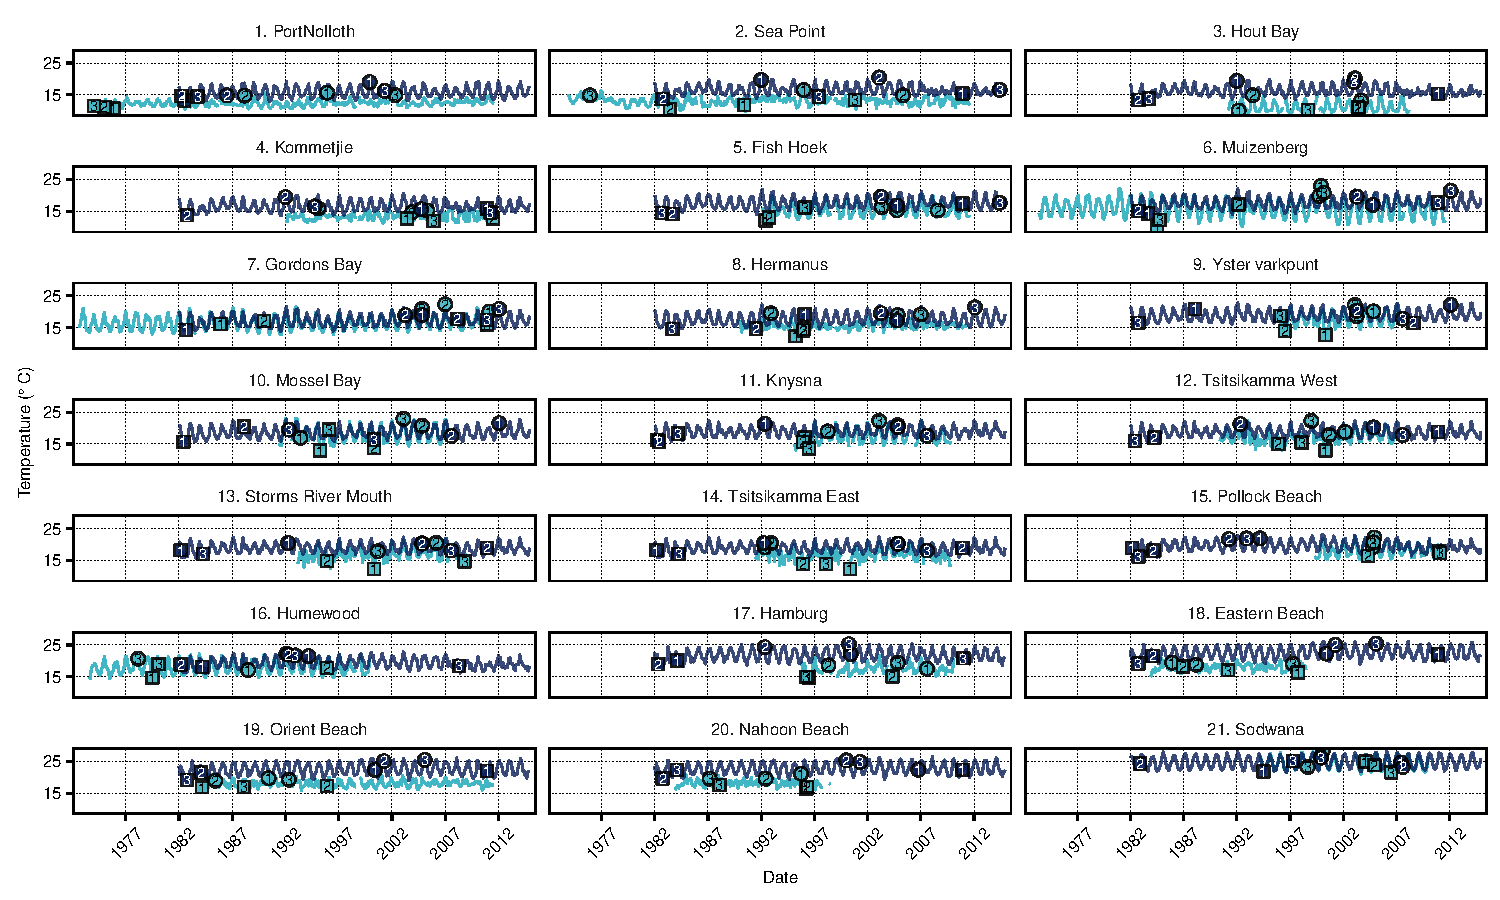
\includegraphics[width=1.0\textwidth]{figure2.pdf}
\caption{The daily temperature values for each \emph{in situ} time series (light blue) used in this study and the corresponding OISST time series (dark blue) extracted for comparison as seen in \Cref{fig:Figure1}. The top three MHWs are indicated by circles (with the rank inside) for each site as judged by greatest cumulative intensity. The top three MCSs for each site are indicated by squares (with the rank inside). Sites 1--4 represent the west coast (WC), sites 5--17 represent the south coast (SC) and sites 18--21 represent the east coast (EC). The coefficient of determination (R$^2$) values for the daily temperatures between each paired set of time series are displayed in the upper left corner of each panel.}
\label{fig:Figure2}
\end{sidewaysfigure}

The daily temperatures on the dates of the largest MHW (MCS) from the west and south coasts in the \emph{in situ} dataset are shown concurrently with the daily temperatures from the OISST time series on matching dates in \Cref{fig:Figure3}. When these largest events were occurring in the \emph{in situ} data, the temperatures in the OISST data did not show similarly intense events.

\begin{figure}
\centering
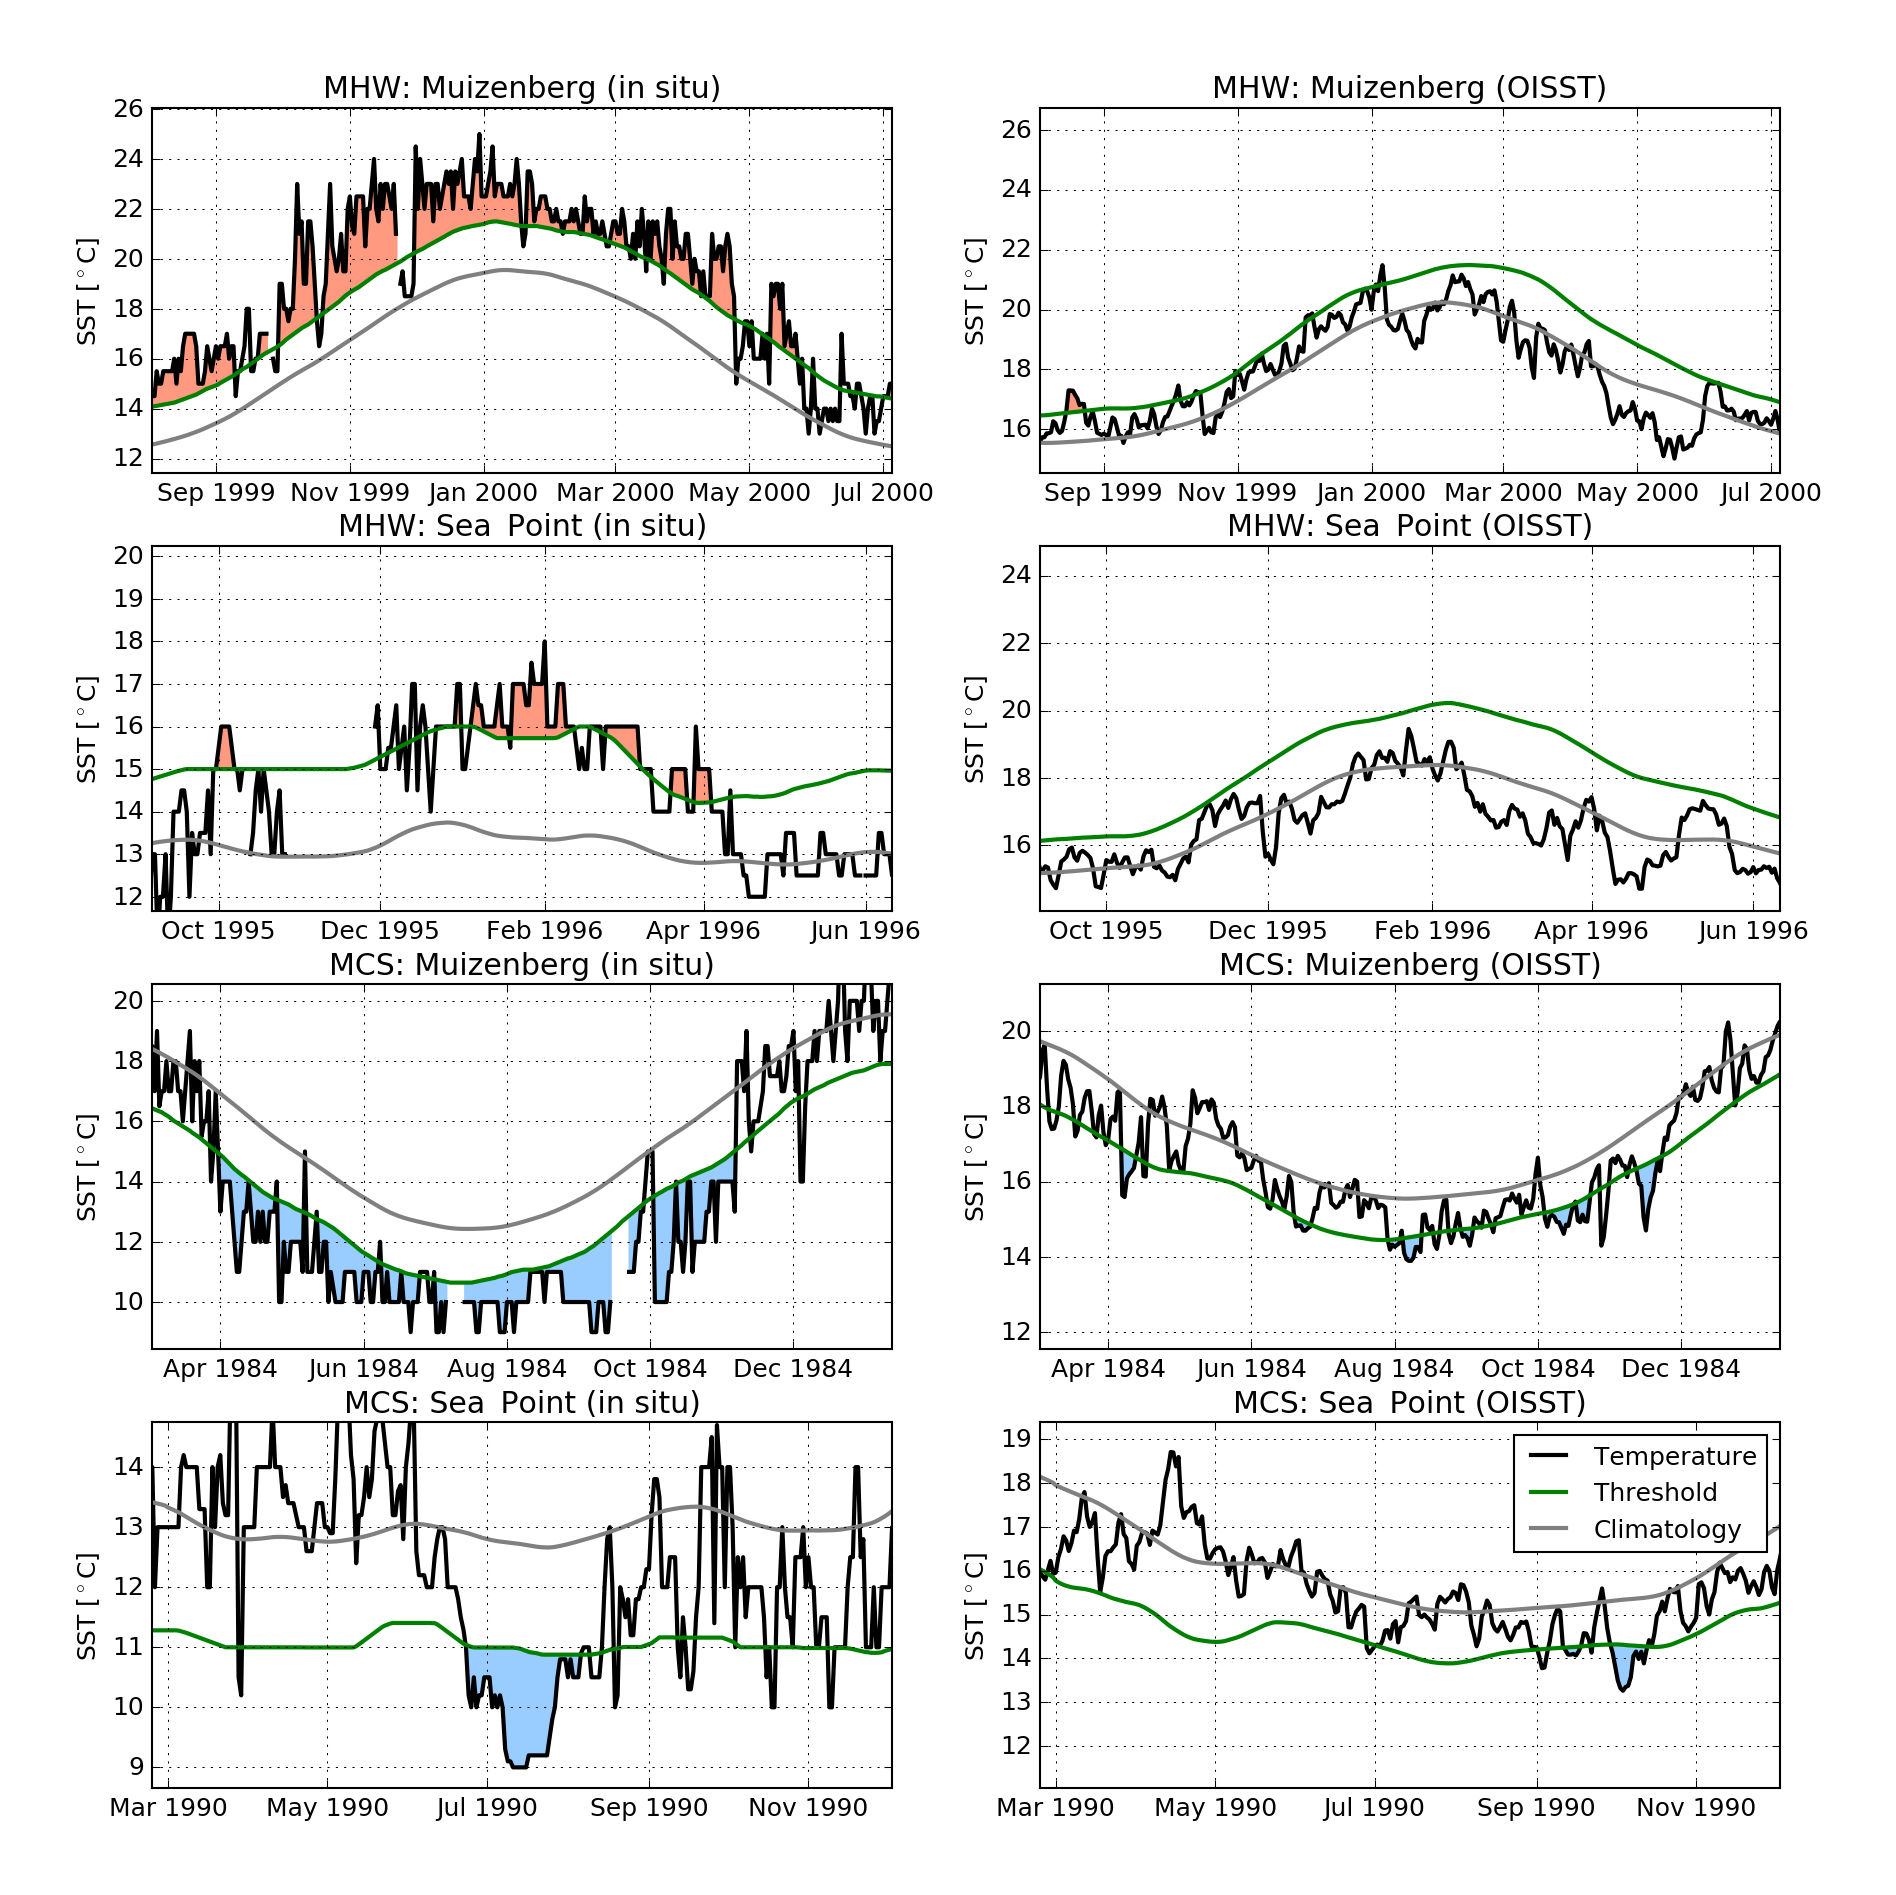
\includegraphics[width=1.0\textwidth]{figure3.png}
\caption{The temperature values from the \emph{in situ} and OISST data during the largest MHW and MCS from the south and west coasts respectively from the \emph{in situ} data. The left column shows the \emph{in situ} temperature values during the event while the right column shows the OISST temperature values occurring on the same dates. The top row shows the largest MHW that occurred on the south coast while the second row shows the largest MHW that occurred on the west coast. The bottom two rows show the largest \emph{in situ} MCS that occurred on the south and west coasts respectively.}
\label{fig:Figure3}
\end{figure}

\subsection{Co-occurrence proportions}
The proportion of co-occurrence found for MHWs (MCSs) between the datasets for each site can be seen in \Cref{fig:Figure4} and \Cref{fig:Figure5} respectively. When using the lag windows both before and after the occurrence of an \emph{in situ} event to compare the \emph{in situ} and OISST events, increasing the width of the lag window from 2 to 14 days caused the mean proportion of co-occurrence for all sites to increase linearly for MHWs (0.09 to 0.38) and MCSs (0.10 to 0.30). Using these same constraints, the south coast sites had the largest mean increase in co-occurrence for MHWs (0.10 to 0.45) and MCSs (0.11 to 0.34), whereas the west coast sites showed the smallest increase for MHWs (0.07 to 0.28) and MCSs (0.08 to 0.19). With all variables controlled for in the same manner, the co-occurrence proportions between the different coastal sections were not significantly different for MHWs or MCSs at 2 day nor 14 day lags (\emph{p}$\geq$0.12).

The directionality of the lag window affected the proportion of co-occurring events. Comparing all events within a 14 day lag window before the \emph{in situ} event gave higher mean (±SD) proportions of co-occurrence for MHWs (0.22±0.13) than for the same lag window after the \emph{in situ} event (0.18±0.10). This same comparison for MCSs showed that the lag window before the \emph{in situ} event (0.16±0.09) had a slightly lower proportion of co-occurrence than the lag window after the \emph{in situ} event (0.17±0.08). When the smaller events were screened from comparison and only the largest half of the events used (50\textsuperscript{th} percentile), the difference in mean (±SD) co-occurrence proportions for MHWs lessened to 0.16±0.11 before the \emph{in situ} event and 0.15±0.12 after. The mean (±SD) co-occurrence proportion of MCSs at this level was less when using a lag window before the \emph{in situ} event at 0.05±0.08 than for a lag window after at 0.08±0.08.

There was no co-occurrence in the paired time series for the largest MCSs, whereas four of the 21 paired time series showed co-occurrence for their largest MHWs (\Cref{fig:Figure4}). Interestingly, these four paired time series were on the south coast and three of the four showed co-occurrence for their largest MHW when the \emph{in situ} event preceded the OISST event.

\begin{figure}
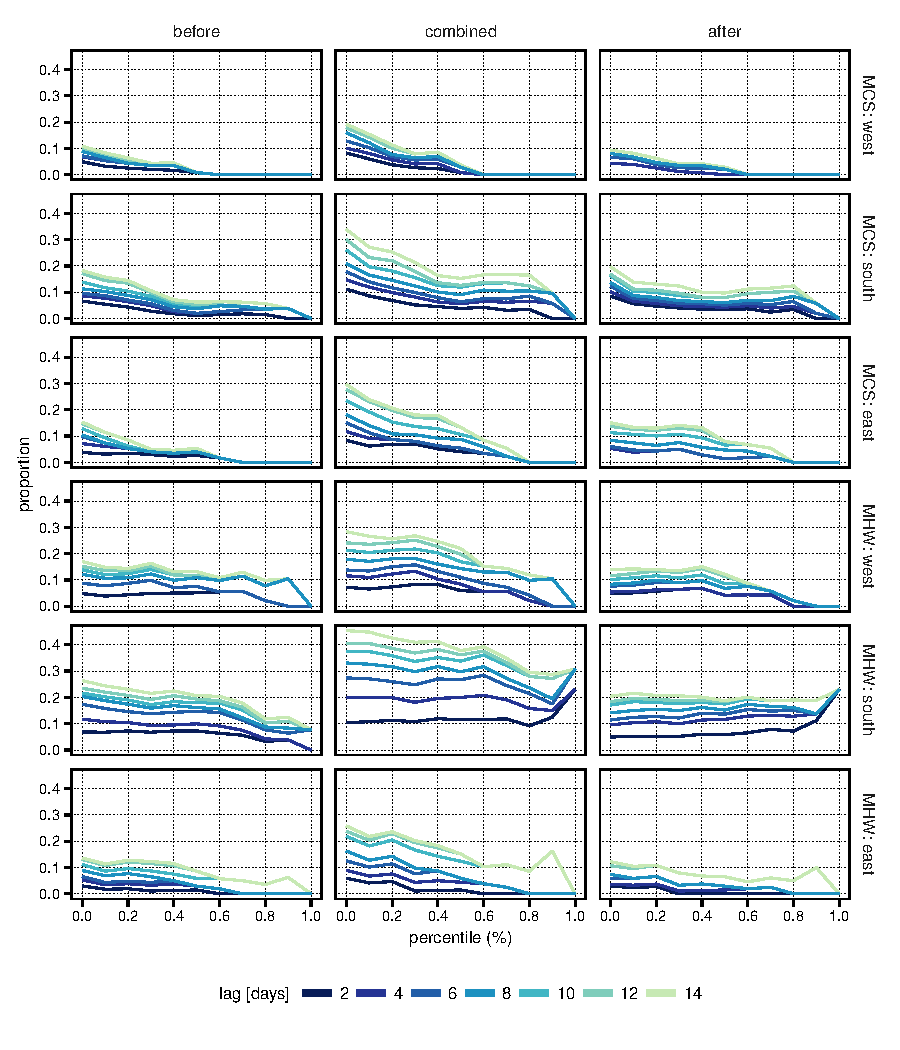
\includegraphics[width=1.0\textwidth]{figure4.pdf}
\caption{Proportion of MHW co-occurrence between \emph{in situ} and OISST datasets for each site where sites 1-4 represent the west coast (WC), sites 5-17 the south coast (SC) and 18-21 the east coast(EC). Columns denoted with ``before'' show the proportion of co-occurrence when events in the OISST data occurred on or before the dates of the \emph{in situ} events. The columns denoted with ``after'' show the proportion of co-occurrence when OISST events occurred after the \emph{in situ} event dates. The $x$-axis indicates the size of the events, based on percentiles, used for calculating the co-occurrence proportions. The days of lag used, from 2-14, are shown here in diminishing shades of red. The numbers above each panel show th ID number for each site. The names of the sites that relate to these ID numbers may be found in \Cref{fig:Figure2} and \Cref{tableS1}.}
\label{fig:Figure4}
\end{figure}

\begin{figure}
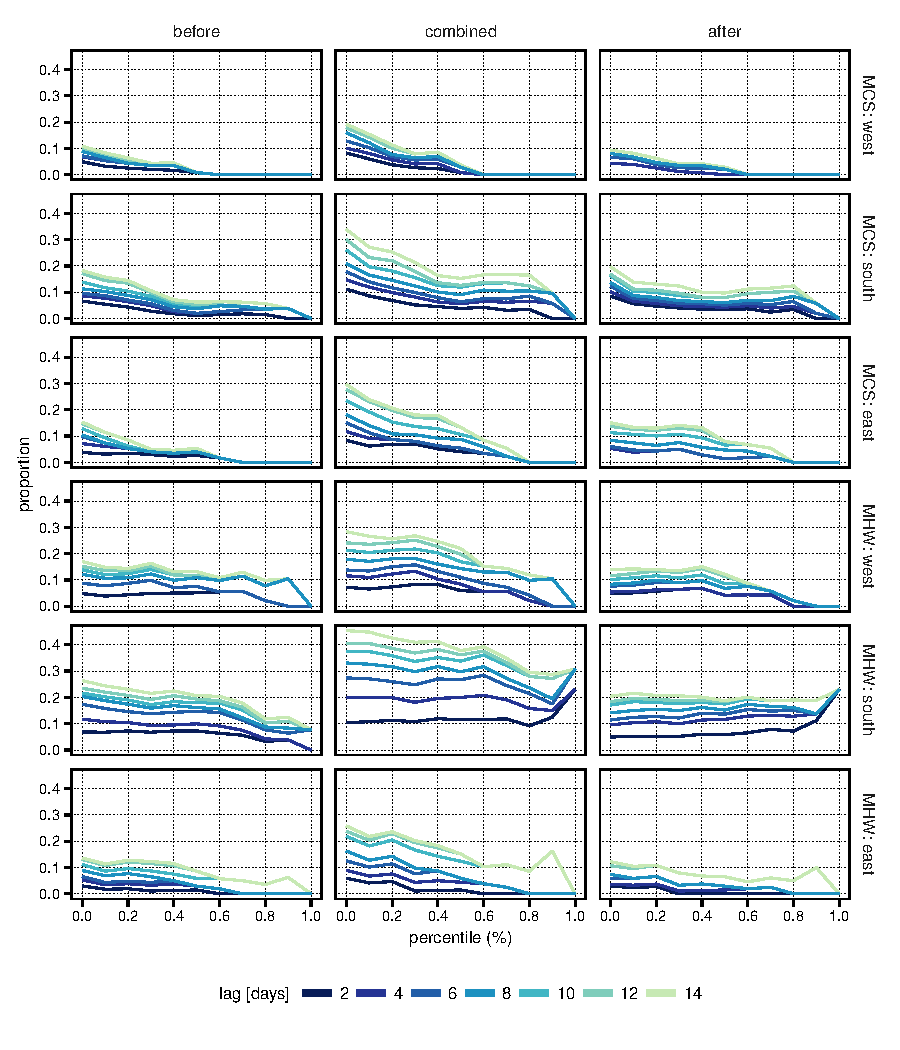
\includegraphics[width=1.0\textwidth]{figure5.pdf}
\caption{Proportion of MCS co-occurrence between \emph{in situ} and OISST datasets for each site as seen for MHWs in \Cref{fig:Figure4}. The days of lag are shown here in diminishing shades of blue.}
\label{fig:Figure5}
\end{figure}

\subsection{Decadal trends in MHWs and MCSs}
The decadal trends in MHWs (MCSs) calculated for each OISST time series are given in \Cref{table4}. The mean (±SD) decadal trend for MHW occurrence in the OISST dataset is 0.2±0.1~dec$^{-1}$ across all sites and -0.3±0.3~dec$^{-1}$ for MCSs. The decadal trends in MHW occurrence were less in the colder Benguela-fed west coast than the warmer Agulhas-driven east coast with the mean (±SD) decadal MHW trend on the west coast being 0.1±0.1~dec$^{-1}$, the south coast being 0.2±0.2~dec$^{-1}$ and the east coast being 0.3±0.1~dec$^{-1}$. Just as MHWs occurred more frequently per decade on the east coast than the west, the count of MCSs decreased more on the east coast than the west. The decadal trend of MCSs on the west coast is 0.0±0.2~dec$^{-1}$, -0.4±0.2~dec$^{-1}$ on the south coast and -0.5±0.2~dec$^{-1}$ on the east coast.

\begin{table}[]
\centering
\caption{\small The results of generalized linear models fitted to the MHW and MCS annual event data of each time series >30 years from the \emph{in situ} (A) and OISST (B) datasets showing the change in extreme events over time. The ID column gives the ID number necessary to locate the site in \Cref{fig:Figure1} and may also be used to find the site name given in \Cref{tableS1}. The coast column shows within which coastal section the time series may be found. The trend columns show the decadal trends of increasing or decreasing extreme events. The \emph{R}\textsuperscript{2} columns shows the coefficients of determination for each general linear model and the \emph{p} columns show the significance of the trend.}
\label{table4}
\begin{tiny}
\begin{tabular}{llccccccc}
\toprule
&& \multicolumn{3}{c}{MHW} & \phantom{abc} & \multicolumn{3}{c}{MCS} \\
\cmidrule{3-5} \cmidrule{7-9}
ID & coast & trend & \emph{R}\textsuperscript{2} & \emph{p} && trend & \emph{R}\textsuperscript{2} & \emph{p} \\
\midrule
{\bf{A} --- \emph{in situ}} \\
1 & west & 0.2 & 0.03 & 0.04 && -0.5 & 0.09 & 0.00 \\
  2 & west & -0.2 & 0.01 & 0.15 && 0.2 & 0.02 & 0.13 \\
  6 & south & 0.1 & 0.00 & 0.68 && 0.2 & 0.03 & 0.06 \\
  7 & south & 0.7 & 0.18 & 0.00 && -0.2 & 0.02 & 0.13 \\
{\bf{B} --- \emph{OISST}} \\
  1 & west & 0.3 & 0.05 & 0.01 && -0.2 & 0.03 & 0.05 \\
  2 & west & 0.1 & 0.00 & 0.55 && 0.1 & 0.00 & 0.57 \\
  3 & west & 0.0 & 0.00 & 0.91 && 0.2 & 0.02 & 0.05 \\
  4 & west & 0.1 & 0.01 & 0.37 && -0.2 & 0.02 & 0.06 \\
  5 & south & 0.3 & 0.04 & 0.02 && -0.6 & 0.14 & 0.00 \\
  6 & south & 0.5 & 0.09 & 0.00 && -0.7 & 0.17 & 0.00 \\
  7 & south & 0.3 & 0.04 & 0.03 && -0.6 & 0.12 & 0.00 \\
  8 & south & 0.4 & 0.07 & 0.00 && -0.6 & 0.13 & 0.00 \\
  9 & south & 0.4 & 0.08 & 0.00 && -0.7 & 0.19 & 0.00 \\
  10 & south & 0.3 & 0.05 & 0.01 && -0.6 & 0.13 & 0.00 \\
  11 & south & 0.3 & 0.03 & 0.04 && -0.4 & 0.07 & 0.00 \\
  12 & south & 0.2 & 0.03 & 0.05 && -0.3 & 0.03 & 0.03 \\
  13 & south & 0.2 & 0.02 & 0.13 && -0.2 & 0.02 & 0.08 \\
  14 & south & 0.2 & 0.02 & 0.13 && -0.2 & 0.02 & 0.08 \\
  15 & south & -0.0 & 0.00 & 0.75 && 0.0 & 0.00 & 0.71 \\
  16 & south & -0.1 & 0.00 & 0.61 && 0.0 & 0.00 & 0.80 \\
  17 & south & 0.1 & 0.00 & 0.45 && -0.4 & 0.04 & 0.01 \\
  18 & east & 0.3 & 0.05 & 0.01 && -0.4 & 0.08 & 0.00 \\
  19 & east & 0.3 & 0.05 & 0.01 && -0.4 & 0.08 & 0.00 \\
  20 & east & 0.2 & 0.02 & 0.06 && -0.3 & 0.04 & 0.02 \\
  21 & east & 0.2 & 0.02 & 0.15 && -0.7 & 0.16 & 0.00 \\
\bottomrule
\end{tabular}
\end{tiny}
\end{table}

Of the four \emph{in situ} time series that reached the 30 year minimum length, the mean (±SD) decadal trend for MHWs is 0.2±0.4~dec$^{-1}$ and -0.1±0.3~dec$^{-1}$ for MCSs. There were two sites from the west coast and two from the south, excluding the east coast from a possible calculation of decadal change for \emph{in situ} MHWs (MCSs). The mean (±SD) decadal trend for MHWs (MCSs) on the west coast is 0.0±0.3~dec$^{-1}$ (-0.2±0.5~dec$^{-1}$) and 0.4±0.4~dec$^{-1}$ (0.0±0.3~dec$^{-1}$) on the south. Note that none of the decadal trends for MCSs from the >30 year \emph{in situ} time series from the west coast were significant.

The mean (±SD) proportion of MHWs that occurred during the second half of the shorter time series was 1.7±1.3 (\emph{p}=0.37) and that of MCSs was 0.8±0.6(\emph{p}=0.39), neither being significantly different. The counts for both MHWs and MCSs between the first and second halves of the time series for the west and south coasts were significantly different. Showing agreement with the longer time series, the short west coast time series had significantly more MHWs in their second half at 1.5±0.6 (\emph{p}=0.03), but differed from the longer time series by having more MCSs in the second half at 1.8±0.6 (\emph{p}<0.01). The short south coast time series showed agreement with the longer time series in that the proportion of MHWs in the second half of time series was greater at 2.1±1.4 (\emph{p}<0.01) and the proportion of MCSs in the second half was lesser at 0.5±0.3 (\emph{p}<0.01). The short east coast time series however, showed no agreement with their longer counterparts. The proportion of MHWs in the second half of these short time series was 0.7±0.4 (\emph{p}=0.10) and the proportion of MCSs was 1.0±0.8 (\emph{p}=0.57).

\subsection{Offshore MHWs and MCSs}
As seen in \Cref{fig:Figure6}, the pixels with the highest annual counts of MHWs occurred well south of the tip of the continent whereas some of the most frequent MCS activity was found directly against the west coast and some small regions of the south coast. As for the duration of events, it is clear from \Cref{fig:Figure6} that the MHWs (MCSs) detected in the Agulhas current are relatively short-lived compared to those in the open ocean with almost all pixels that showed events in the upper range of duration detected well away from the coast. The offshore events along the west and south coasts have centers of intensity very near the shore whereas the east coast generally does not. The most intense events detected in the OISST data are found along or south of the south coast.

\begin{figure}
\centering 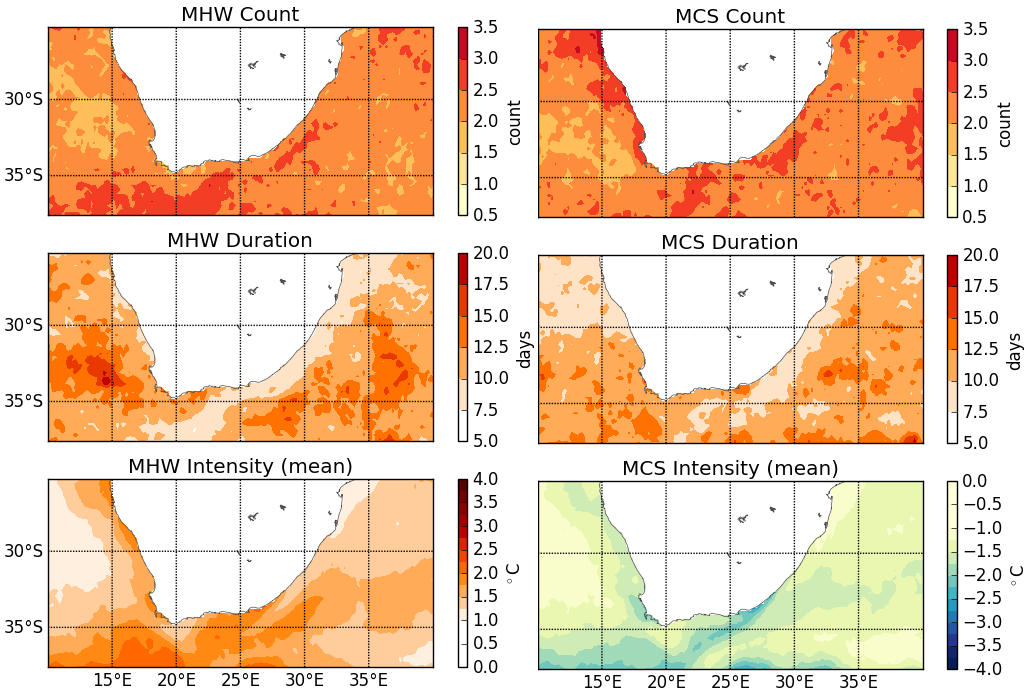
\includegraphics[width=1.0\textwidth]{MHW_MCS_mean.png}
\caption{Mean values from the annual data of each pixel from the OISST dataset around southern Africa. The first second and third rows show the mean count [n], duration [days] and intensity [\degree C] respectively of MHWs in the first column and MCSs in the second. The annual event values within each pixel were averaged to create one final value with which each pixel is populated.}
\label{fig:Figure6}
\end{figure}

Whereas the mean count, duration and intensity of MHWs and MCSs offshore are telling, the picture is not complete without also considering the trend in these metrics, too. \Cref{fig:Figure7} shows that the count, duration and intensity of MHWs increased almost exclusively throughout the studied regions of the Indian and Atlantic Oceans. The count of MCSs decreased most rapidly along the coast of southern Africa with a couple of notable exceptions near Port Elizabeth and north of the Cape Peninsula where the count of MCSs increased very near to the coast. The duration of MCSs is seen to have generally increased further offshore with most of the nearshore region having changed little or decreased. The intensity of MCSs either changed little near the coast or increased dramatically, as seen in the dark blue spot north of the Cape Peninsula in the ``MCS Intensity (mean) Trend'' panel in \Cref{fig:Figure7}.

\begin{figure}
\centering 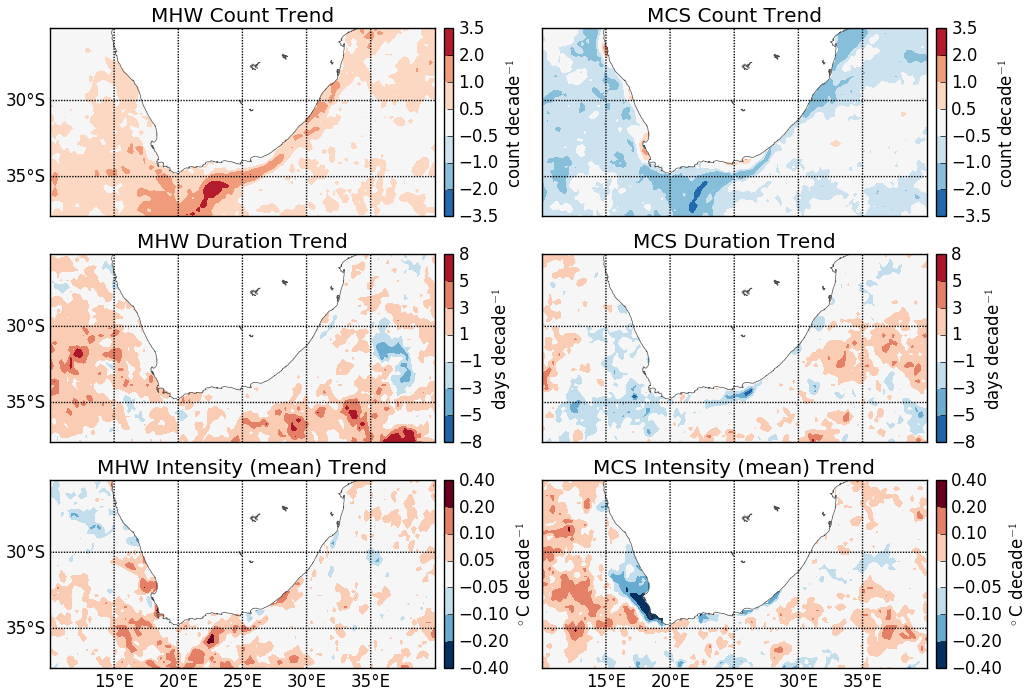
\includegraphics[width=1.0\textwidth]{MHW_MCS_trend.png}
\caption{Decadal trend values calculated from the annual OISST data around southern Africa. The decadal trends were calculated by fitting a linear model to the annual data of each pixel for the relevant metrics and multiplying the slope of the line by 10. The panels are in the same position as \Cref{fig:Figure6}.}
\label{fig:Figure7}
\end{figure}

\section{Discussion}
Our results clearly show that MHWs (MCSs) detected in two different ocean temperature datasets displayed markedly different counts, durations, intensities and timing in their occurrence. These differences appear to be related to the nature and variability of physical oceanographic processes at broad- and local-scales, and the coupling of the processes across these scales. These finding illustrate how a study of the properties of anomalous events can provide novel insights into drivers of the thermal regime along coastlines, and can be used to arrive at some mechanistic insights into the nature and origin of MHWs (MCSs).

\subsection{Relation between local- and broad-scale MHWs and MCSs}
The difference between the \emph{in situ} and OISST datasets was striking. We anticipated a large degree of coupling between MHWs manifesting in datasets that encapsulate local- and broad-scale patterns, as represented by the \emph{in situ} and OISST datasets, respectively. We found instead that the broad-scale dataset yielded heatwaves that were more frequent and longer in duration, but less intense than their local-scale counterparts. Cold-spells, for which we expected a greater deal of decoupling between local- and broad-scale manifestations, showed more evidence of such than MHWs. MCSs were more frequent and lasted longer in the OISST data; however, the mean intensity of MCSs at the broad-scale was less than at the local-scale. The significantly larger intensities of both MHWs and MCSs from the \emph{in situ} data may be an artifact of the inability of remotely sensed data to record the maximum and minimum temperatures that \emph{in situ} instruments are capable of detecting \citep{Smale2009}.

Such a deterioration of the offshore thermal signal in coastal waters is known to occur due to the local modifications of nearshore circulation patterns by headlands, embayments, influences of the bathymetry and other such perturbations that introduce eddies and fronts and a shoaling of the thermocline \citep{Okubo1973, Pingree1979, Wolanski1988, Black1990, Grundlingh1991, Graham1997}. These processes are not yet fully understood, and what understanding we do have of physical oceanographic process remains weighted toward the mesoscale, as was noted by \citet{Graham1997} in their study on upwelling shadows, another process responsible for the local modification of a phenomenon that is generally studied at the broad-scale. These local-scale deviations are known to affect coastal ecological processes, such as the transport, dispersal and settlement of larvae \citep{Pineda1994, McCulloch2003, Narvaez2004} and the dynamics of phytoplankton and nutrient delivery \citep{Graham1997, Pineda1994}, and it is likely that thermal patterns over similar scales will also have local significance for nearshore biology.

\subsection{MHWs and MCSs in different coastal sections}
There was no difference in the annual count of events between coasts within each dataset (\Cref{table1}) but the duration and intensity metrics between coasts did differ. An important thing to note from \Cref{table1} is that the MHWs and MCSs at both the local- and broad-scale on the east coast were significantly shorter in duration than other two coastal sections; however, comparing the event duration between events, we see that on this coast the cold-spells lasted longer than heatwaves in the OISST data. Furthermore, the east coast also displayed the least intense MHWs but most intense MCSs of any coastal section in the OISST dataset. This stretch of coastline is heavily influenced by the warm Agulhas Current, separated from the coast only by a very narrow and steep continental shelf, which abruptly expands into the >200km wide Agulhas Bank south of Port Alfred (\Cref{fig:Figure1}). This narrow continental slope margin allows upwelling on the shoreward side of the Agulhas Current to occur along the entire length of the east coast, independent of local atmospheric conditions \citep{Lutjeharms2000}. It is therefore possible that this constant forcing of the Agulhas Current on the east coast would cause the events arising there to dissipate more quickly and return to a `normal,' less variable state. This seems to be a plausible explanation for why the largest events, both hot and cold, recorded on the east coast are so much smaller than those along the other two coastal sections. We suggest that the hydrodynamic properties of the Agulhas Current have prevented any prolonged temperature events from persisting. Contrary to this conclusion it is clear from the literature that some of the largest documented heatwaves have been caused by anomalously high heat content of ocean currents, such as the Leeuwin Current in the case of the Western Australia MHW \citep{Feng2013, Pearce2013, Wernberg2013}. Conversely, large MHWs such as that documented in the north west Atlantic Ocean in 2012 have been shown to be coupled strongly with atmospheric phenomena \citep{Mills2012, Chen2014, Chen2015}. Therefore, while no MHWs or MCSs with cumulative intensities rivaling those of the largest events seen on the other two coasts have yet occurred on the east coast, the potential exists for some further-afield phenomenon to cause such an event there.

Some of the \emph{in situ} time series collected along the south coast are recorded in relatively shallow embayments, allowing for atmospheric heating to have a marked effect there --- as is indeed seen in the cumulative intensities for MHWs in False Bay --- and further offshore sheer-edge forcing creates eddies resulting from the departure of the Agulhas Current from the Agulhas Bank that may then be projected across the shelf \citep{Lutjeharms2003}. Such high temperature events last longer, and even if their mean intensities are lower, this contributes towards their high cumulative intensities. The significantly more intense nearshore MCSs on the south coast are attributed to the much greater mean intensity of events around Tsitsikamma (Sites 12--14). Without these three sites the nearshore MCSs on the south coast are not significantly greater than those along the other two coastal sections. \citep{Roberts2005} hypothesized that a wind forced upwelling cell occurs near Tsitsikamma and the mean intensity of the events recorded here may support this.

The west coast does not show exceptional patterns in MHW and MCS metrics. At first glance, we were surprised to find that the mean intensity of west coast (EBUS) coastal MCSs is lower than those on the south coast. Upwelling systems are defined by periodic occurrences of cold water of deep origin near the coast \citep{Lutjeharms2000, Hutchings2009} and it seems intuitive to associate these with the cold-spells. But cold upwelled water \emph{defines} the climatology for the region, and for a cold-spell to manifest in an upwelling region the temperature of that water would have to be colder than the 90th percentile based on a 30-year climatological baseline period and would have to last for five or more days. Accordingly, upwelling events that occur within a seasonally predictable cycle are not anomalous in nature, and are therefore not flagged as MCSs. An upwelling event would need to be particularly cold or a-seasonal in its occurrence to be recorded as a MCS. This is certainly possible; however, the very nature of the required a-seasonality of MCSs obfuscates which phenomena may potentially be driving the extreme cold temperatures. This consideration casts doubt on our thoughts to use MCSs as a means to detect the intensification of upwelling, which is a plausible prediction in an age when Earth's climate gradually warms \citep{Garcia-Reyes2015}. Results show that offshore MCS are, on average, lasting significantly longer, occurring significantly more often and the largest events are more intense. As upwelling is known to occur along the coast here \citep{Hutchings2009}, that the offshore MCSs occur more often and last longer is strong evidence that the MCS algorithm is not a good proxy for upwelling detection and that the coastal cold events detected here are likely due to other factors. Upwelling events should have notable properties, such as rate of onset and duration of peak intensity, which set them apart from other events that may cause colder water to occur at the surface. Further work on the definition of the characteristics of upwelling events could be coupled with the MCS algorithm for accurate use in upwelling detection in temperature time series.

\subsection{Patterns in mean cumulative intensity}
The pattern of mean cumulative intensity within the local-scale data was very clear in that warm and cold events on the south coast were much more extreme than those along the west and east coasts. The OISST data were less conclusive on whether the south or west coast experienced the most extreme events, but it is apparent from all of the analyses from both datasets that the east coast experienced very few extreme MHWs or MCSs. These findings suggest that the east coast is the most thermally stable of the three coastal sections, and that MHWs or MCSs with mean cumulative intensities that could potentially damage ecosystems are least prone to develop there. It is the south coast region, however, where coastal ecosystems are most at risk due to excessively warm events.

Within the south coast (Sites 5--17), the sites within False Bay (Sites 5--7) have greater cumulative intensities for MHWs and MCSs than the sites over the Agulhas Bank (Sites 8--17). Whereas the Agulhas Bank experiences more thermal variation than the other two coastal sections, False Bay, which is \textasciitilde50 km across, is situated within the transition zone between the Benguela and Agulhas Currents \citep{Smit2013} and contains the most variable time series in the entire \emph{in situ} dataset. Lower resolution satellite temperature products, such as Pathfinder version 5.0, have been shown to inadequately resolve the SST within the relatively small body of water that is False Bay \citep{Dufois2012}. Embayments such as this often display thermal ranges (both temporally and spatially) large enough to effect species ranges \citep{Ling2009} and are of great ecological \citep{Klumb2003} and economic importance \citep{Lugendo2005}. We think that such regions are also more prone to MHWs (and perhaps MCSs) due to an even stronger decoupling from broad-scale thermal patterns and drivers: indeed, two of the three largest MHWs and MCSs detected in the local-scale dataset were recorded within False Bay, whereas only one large MHW and no MCSs were detected there within the OISST dataset. This illustrates the problem of using satellite temperature data for coastal ecological applications, and emphasizes the need for more comprehensive coverage of nearshore ecosystems in long-term \emph{in situ} seawater temperature monitoring programmes.

Although \citet{Hobday2016} provide caveats regarding using event metrics across datasets, we nevertheless feel that it would be informative to bring the heatwave metrics measured along the South African south coast into context by comparing them with MHWs from regions \citep[see][]{Hobday2016}. We see that at our coastal locations, Muizenberg and Mossel Bay, heatwaves have \emph{on average} cumulative intensities ranging from 156.4 to 310.30 \degree C$\cdot$days, mean intensities from 1.77 to 4.47 \degree C and lasting from 35 to 98 days. The two longest individual MHW events experienced by the Western Australian reef system \citep{Feng2013} had a cumulative intensity of 237 \degree C$\cdot$days, a mean intensity of 2.5 \degree C and a duration of 95 days in 1999; and a cumulative intensity of 276 \degree C$\cdot$days, a mean intensity of 2.51 and a duration of 110 days (and ongoing at the time of their analysis) in 2014. The 2012 MHW of the north west Atlantic \citep{Mills2012, Chen2014} had a cumulative intensity of 145 \degree C$\cdot$days and mean intensity of 4.00 \degree C over 56 days, while the subsequent 2012/2013 heatwave went to 443 \degree C$\cdot$days and a mean intensity of 2.59 \degree C and lasted for 187 days. Both of these MHWs were reported to have had major ecological consequences \citep{Feng2013, Mills2012, Chen2014}, but no investigations have yet been done to see if similar negative effects have taken place at the sites where we have recorded intense heatwaves locally. Probably none have occurred as evidence for such do not exist amongst the fisheries survey data collected annually, but a more detailed investigation is warranted to see if \emph{some} of the ecological changes known for the south coast region \citep{Bolton2012} can be linked to such events. Nevertheless, considering that the south coast is a `hot-spot' for heatwaves, the fact that these events are increasing in count and knowledge that events already experienced in the region are already on par with the intensity and duration of similar events known to have had ecological effects elsewhere in the world, it is a matter of time before South Africa experiences a similar marine environmental `natural' disaster.

\subsection{Co-occurrence proportions}
We found that the majority of the events in the paired time series between the two datasets were unrelated and that some other influence(s) could have had a more pronounced effect on the nearshore events than offshore temperatures. This finding is important in light of the very strong mismatch in temperatures recorded by thermal loggers installed \emph{in situ} at the coast (i.e. local-scale) compared to measurements of the ocean's temperature from space (i.e. broad-scale) \citep{Smit2013}.

When isolating co-occurrence proportions between the datasets to OISST events preceding \emph{in situ} events, we see that the proportions of co-occurrence for MCSs were much lower than for MHWs (\Cref{fig:Figure4} and \Cref{fig:Figure5}). This shows that if co-occurring events are indeed related, more MHWs are being caused by mesoscale activity than MCSs, as was expected. Additionally, more MCSs from the OISST data were shown to occur after \emph{in situ} MCSs for all coastal sections. This may suggest some local heat loss process, perhaps related to atmospheric cold events, cooling the waters near the coast, which then spread to waters further offshore. The co-occurrence proportions of OISST MHWs before and after \emph{in situ} MHWs are similar, implying that MHWs may be just as likely to propagate onshore from offshore mesoscale activity as MHWs originating near the coast may seep offshore and affect the thermal regime there.

We also infer from the proportions of co-occurrence of time series on the south coast, which are generally much higher than at the other two coasts, that events are caused by the much higher level of influence from mesoscale phenomena occurring over the Agulhas Bank. We also see that there is a higher proportion of co-occurrence for the larger MHWs and MCSs on the south coast when a lag window after the \emph{in situ} event is applied. This supports the argument that events originating in the nearshore are propagating out onto the Agulhas Bank and affecting the oceanography there more often than offshore events originating on the Agulhas Bank are affecting the nearshore environment. However, the overall low rate of co-occurrence for all three coastal sections reinforces the argument that it is not the mesoscale phenomena of the open ocean abutting the southern African landmass that are driving events in the nearshore.

The decline in the proportions of co-occurrence between datasets as the smaller events are screened out is strong evidence against the hypothesis that mesoscale activity, both warm and cold, is causing nearshore thermal events. The small increases in co-occurrence for some sites as only larger events were compared does imply that there is some relationship between the nearshore and offshore at some localities, but that some other variable (e.g. atmospheric forcing) may be having a greater effect on nearshore events.

Another important consideration is the co-occurrence of the events with the highest mean cumulative intensity within and between datasets. None of the dates for the top three MHWs or MCSs for any of the coastal sections from the \emph{in situ} dataset are the same (\Cref{table3}). They are all individually different events occurring at different times. The OISST dataset tells an entirely different story in that all but one of the coastal sections, for both MHWs and MCSs, have at least two of their three top events occurring at the same time. This means that the largest events detected in the OISST dataset occur over a broad area at the same time, whereas the \emph{in situ} events are isolated temporally and spatially. This further reinforces our conclusion that the events detected by the different datasets are often intrinsically different from one another.

A final consideration to address for the apparent lack of relation between these datasets is that the OISST temperatures are remotely sensed representations of the surface and though they are converted from a ``skin'' temperature (roughly a micron deep) to a ``bulk'' temperature (roughly half a meter deep) \citep{Reynolds2007}, 7 of the 21 time series from the \emph{in situ} dataset were recorded deeper than this with 2 of them recorded deeper than 10 meters. However, these deeper \emph{in situ} data are still comparable to the "bulk" upper mixed layer the OISST data are calibrated to measure as there is little vertical layering within the nearshore environment. Furthermore, the OISST temperatures are averaged across the width of the continental shelf at each site, and not simply to the nearest available pixel, largely addressing any inconsistencies in temperature caused by mismatches in depth as the mixed layer of the mesoscale temperature patterns of the open ocean should be comparable in depth to the nearshore water column. It is then worth noting that water temperatures being measured in the \emph{in situ} dataset represent the area where the nearshore biota are living, and is better able to reflect what temperature patterns/ exposure these flora and fauna experience. Therefore two datasets are necessary: one for the coast; one for the ocean. The aim is not to compare the accuracy of the two datasets to detect the same events, rather this study aims to show that fundamentally different outcomes exist, and that in order to show the vulnerability of nearshore ecosystems to climate change, an appropriate dataset must be used.

\subsection{Climate change}
Although all but four of the \emph{in situ} time series used in this investigation are too short to draw adequate conclusions on the decadal trends seen in MHWs and MCSs, the OISST time series are long enough. As hypothesized, these data show positive decadal trends for MHWs and negative trends for MCSs. This means that over the past 33 years of satellite observation, MHWs have been increasing every decade for each coastal section while MCSs have been decreasing. Whereas the literature surrounding the potential increase (decrease) of MHWs (MCSs) in the ocean is still in its infancy, atmospheric scientists have been investigating the shift in extreme events for over a decade. Both historic and modelled research shows that climate change is leading to an increase of extreme hot events in the atmosphere \citep{Easterling2000, Perkins2013}, and decreasing extreme cold events \citep{Meehl2004}. It is not surprising to find the same pattern in the ocean as seen \Cref{fig:Figure7}.

Though less conclusive than the trends calculated from the longer time series, similar patterns were found in the shorter \emph{in situ} time series as well. As the algorithm used to calculate these events is based on percentiles, it stands to reason that as the mean temperature of the oceans has been increasing by roughly 0.1\degree C per decade on average over the past several decades \citep{IPCC2014}, there will be an increase in MHWs and a decrease in MCSs. The gradual mean increase in temperature will cause the algorithm used here to be biased in its detection of MHWs as time progresses simply because temperatures are generally warmer in the later half of the time series therefore, the chances of the algorithm detecting a MHW increases because the base temperature from which the MHW will be fluctuating from will be greater than the beginning of the time series. Ultimately, for the species and ecosystems experiencing this increase in duress, the semantic argument of the viability of percentiles provides little solace.

\section{Conclusion}
Given that the MHW algorithm is based on the percentiles found within each time series and not on predetermined minimum or maximum thresholds, one will always find MHWs and MCSs in any time series. It is our experience with these data that every time series used from both datasets experienced, on average, at least one MHW and MCS per year. Within each dataset, but not between, the count of events is similar for each coastal section, regardless of the local oceanographic and geographic properties. Instead, it is the duration, mean intensity and also the derived cumulative intensity of the events occurring on the different coastal sections that most clearly define spatial differences --- so much so, that this will almost certainly translate to different rates of vulnerabilities of coastal sections, both the ecosystems and the humans that derive benefit from them, to the ravages of climate change. As the proportion of co-occurrence of events between the local- and broad-scale dataset are generally low, and the magnitude of events within the different datasets differ significantly from one another, we infer that some other force outside of mesoscale temperature phenomena is contributing to nearshore events. We think that direct atmospheric forcing of coastal thermal heating is one such driver that needs immediate research attention in order to better understand what is driving the occurrence and intensity of these events.

Of the metrics presented in this paper, cumulative intensity is perhaps the most important ecologically. As a product of the intensity and duration of an event, we propose that cumulative intensity may be used as an index to measure the threat of thermal events to coastal ecosystems. Future research conducted on damaging MHWs and MCSs will be able to record the cumulative temperature above the seasonal average experienced by the ecosystem in question. As the body of research on extreme events increases, the aggregated cumulative intensity values may be used to establish a global index of the thresholds for different ecosystems at which ecological perturbations, impairment or destruction have occurred. Combined with near real time monitoring, this metric may then be used to improve the decision making process on how when and how best to respond to unusually warm or cold bodies of water. Furthermore, we found in this study that the cumulative intensity of events at the coast were not only greater than the corresponding OISST events, but that the upper range was much greater.

We have provided a cursory look at an oceanographic basis for explaining these differences, but we think that there is an urgent need to consider more carefully the complex local-scale modifications of broader-scale patterns seen further afield in order to fully appreciate the drivers of coastal thermal variability in space and time. That such studies are still lacking in an age when the pulse of the global ocean is measured with exquisite precision is a reflection on the oceanographic community's ongoing preoccupation with mainly broad-scale open ocean patterns and processes. Globally comprehensive ocean temperatures are made available almost in real time, but to the best of our knowledge the top coastal temperature databases are all comprised of records retrieved from delayed-mode instruments. In the latter case, near-real-time warnings of the onset and intensity of MHWs (or MCSs) are not yet feasible, whereas it is already possible to develop and implement such warning systems using currently-available gridded satellite SST products. Researchers in the tropics, on coral reefs specifically, are already doing just this as they implement (near) real-time satellite data for the monitoring of coral bleaching (e.g. http://coralreefwatch.noaa.gov/satellite/index.php). Other coastal communities should learn from the work of tropical communities in implementing monitoring systems for extreme temperatures, which is now becoming relevant as climate change is threatening previously (relatively) stable ecosystems, such as temperate kelp forests \citep{Wernberg2016}. We therefore feel that there is a need to begin implementing near-real-time montioring systems so that we may track the benefits of these systems in terms of prediction, detection and mitigation of the potential damage caused by extreme events. Furthermore, we propose that the focus of this implementation be on nearshore ecosystems as these are disproportiantely more important to human livelihoods as well as being at greater risk generally than other marine ecosystems.

\section*{Acknowledgements}
We would like to thank DAFF, DEA, EKZNW, KZNSB, SAWS and SAEON for contributing all of the raw data used in this study. Without it, this article and the South African Coastal Temperature Network (SACTN) would not be possible. This research was supported by NRF Grant (CPRR14072378735) and by the Australian Research Council (FT110100174). This paper makes a contribution to the objectives of the Australian Research Council Centre of Excellence for Climate System Science (ARCCSS). The authors report no financial conflicts of interests. The data and analyses used in this paper may be found at https://github.com/schrob040/MHW.

\newcommand{\beginsupplement}{%
        \setcounter{table}{0}
        \renewcommand{\thetable}{S\arabic{table}}%
        \setcounter{figure}{0}
        \renewcommand{\thefigure}{S\arabic{figure}}%
     }
\beginsupplement

\section*{Supplementary}
\subsection*{Meta-data}
Further meta-data for each time series and source listed in geographic order along the South African coast from the border of Namibia to the border of Mozambique may be found in \Cref{tableS1}.

\begin{table}[]
\caption{\small The metadata and coastal averages for all \emph{in situ} time series used in this study.}
\label{tableS1}
\centering
\tiny
\begin{tabular}{cllcccccccccc}
  \hline
 ID & site & coast & lon & lat & start date & end date & duration (years) & NA \% & mean & sd & min & max \\
  \hline
1 & Port Nolloth & west & 16.87 & -29.25 & 1973-07-22 & 2011-08-31 & 38.1 & 6.8 & 12.3 & 1.4 & 9.2 & 21.0 \\
2 & Sea Point & west & 18.38 & -33.92 & 1973-12-31 & 2011-08-10 & 37.6 & 6.3 & 13.1 & 1.6 & 8.7 & 23.0 \\
3 & Hout Bay & west & 18.35 & -34.05 & 1991-03-25 & 2008-04-21 & 17.1 & 4.9 & 11.2 & 1.8 & 7.5 & 16.7 \\
4 & Kommetjie & west & 18.33 & -34.14 & 1992-02-29 & 2011-08-17 & 19.5 & 7.4 & 13.3 & 1.6 & 9.0 & 20.4 \\
coast & mean & west &  &  &  &  & 28.1 & 6.3 & 12.5 & 1.6 & 8.6 & 20.3 \\
5 & Fish Hoek & south & 18.44 & -34.14 & 1992-02-29 & 2011-08-17 & 19.5 & 5.9 & 15.4 & 2.3 & 10.0 & 22.5 \\
6 & Muizenberg & south & 18.48 & -34.10 & 1973-05-04 & 2011-08-24 & 38.3 & 3.9 & 15.9 & 3.0 & 9.0 & 25.0 \\
7 & Gordons Bay & south & 18.86 & -34.16 & 1972-09-12 & 2011-08-24 & 39.0 & 4.0 & 16.5 & 2.4 & 10.0 & 25.5 \\
8 & Hermanus & south & 19.25 & -34.41 & 1989-11-30 & 2011-05-18 & 21.5 & 4.1 & 15.6 & 1.6 & 9.0 & 23.5 \\
9 & Ystervarkpunt & south & 21.74 & -34.40 & 1995-10-23 & 2007-06-19 & 11.7 & 0.0 & 17.6 & 2.6 & 10.1 & 23.6 \\
10 & Mossel Bay & south & 22.16 & -34.18 & 1991-06-26 & 2007-06-19 & 16.0 & 8.4 & 18.0 & 2.7 & 10.1 & 24.6 \\
11 & Knysna & south & 23.07 & -34.08 & 1995-03-21 & 2009-11-04 & 14.6 & 6.3 & 17.3 & 2.6 & 10.7 & 24.2 \\
12 & Tsitsikamma West & south & 23.65 & -33.98 & 1990-06-30 & 2007-02-14 & 16.6 & 7.7 & 17.2 & 2.6 & 9.5 & 29.3 \\
13 & Storms River Mouth & south & 23.90 & -34.02 & 1993-03-31 & 2008-12-30 & 15.8 & 4.0 & 16.8 & 2.5 & 9.4 & 24.4 \\
14 & Tsitsikamma East & south & 23.91 & -34.03 & 1991-06-29 & 2009-11-08 & 18.4 & 4.0 & 16.8 & 2.5 & 8.8 & 23.4 \\
15 & Pollock Beach & south & 25.68 & -33.99 & 1999-05-12 & 2011-07-06 & 12.2 & 3.0 & 18.1 & 2.1 & 10.8 & 26.5 \\
16 & Humewood & south & 25.65 & -33.97 & 1973-08-24 & 1999-12-30 & 26.4 & 3.1 & 18.0 & 2.3 & 11.0 & 25.0 \\
17 & Hamburg & south & 27.49 & -33.29 & 1995-10-30 & 2010-02-25 & 14.3 & 6.4 & 17.5 & 1.8 & 12.1 & 24.1 \\
coast & mean & south &  &  &  &  & 20.3 & 4.7 & 17.0 & 2.4 & 10.0 & 24.7 \\
18 & Eastern Beach & east & 27.92 & -33.02 & 1983-12-31 & 1998-07-30 & 14.6 & 9.8 & 17.9 & 1.8 & 12.5 & 25.0 \\
19 & Orient Beach & east & 27.92 & -33.02 & 1983-12-31 & 2011-07-06 & 27.5 & 3.9 & 18.0 & 1.6 & 12.0 & 26.0 \\
20 & Nahoon Beach & east & 27.95 & -32.99 & 1983-12-31 & 1998-07-30 & 14.6 & 7.0 & 18.1 & 1.7 & 10.0 & 25.0 \\
21 & Sodwana & east & 32.73 & -27.42 & 1994-03-11 & 2010-01-25 & 15.9 & 7.0 & 24.4 & 2.0 & 18.6 & 29.1 \\
coast & mean & east &  &  &  &  & 18.2 & 6.9 & 19.6 & 1.8 & 13.3 & 26.3 \\
   \hline
\end{tabular}
\end{table}

\section*{References}

% Disable the following line when wanting to repopulate the .bbl file from the MHW.bib file
%\bibpunct{(}{)}{;}{a}{}{,} % Not certain this line is necessary...

\bibliography{MHW} % Comment out when manually copying the references from the .bbl file
% Delete all of the following when using the MHW.bib file with the above line
% No one here but us chickens...
% Delete the above line when using the MHW.bib file instead of copying in the .bbl file

\end{document}